\protect\hypertarget{anchor}{}{}
\includegraphics[width=2.9839in,height=1.4925in]{./media/Pictures/1000020100000640000003207F00E813C54DBA79.png}
\includegraphics[width=1.9398in,height=1.3425in]{./media/Pictures/1000020100000190000001152E304599A0C7AC42.png}

\protect\hypertarget{anchor-1}{}{}

\protect\hypertarget{anchor-2}{}{}\textbf{Idiomatic Programmer}

\protect\hypertarget{anchor-3}{}{}\textbf{Handbook Primer: Fundamentals
of Statistics}

\protect\hypertarget{anchor-4}{}{}\textbf{Andrew Ferlitsch, Google AI\\
}Version July 2019

\protect\hypertarget{anchor-5}{}{}

\protect\hypertarget{anchor-6}{}{}\textbf{The Idiomatic Programmer -
Statistics Primer}

\protect\hypertarget{anchor-7}{}{}Handbook Primer - Fundamentals of
Statistics

\emph{Part A - Basic Statistics}

\emph{Part B - Linear/Logistic Regression}

\emph{Part C - CART Analysis}

\emph{Part D - Conditional Probabilities}

\protect\hypertarget{anchor-8}{}{}\textbf{Part A - Basic Statistics}

As a Googler, one of my duties is to educate software engineers on how
to use machine learning. I already had experience creating online
tutorials, meetups, conference presentations, and coursework for coding
school, but I am always looking for new ways to effectively teach.

Welcome to my latest approach, the idiomatic programmer. My audience are
software engineers who are proficient in non-AI frameworks, such as
Angular, React, Django, etc. You should know at least the basics of
Python. It's okay if you still struggle with what is a compression, what
is a generator; you still have some confusion with the weird
multi-dimensional array slicing, and this thing about which objects are
mutable and non-mutable on the heap. For this tutorial it's okay.

You have a desire (or requirement) to become a machine learning
engineer. What does that mean? A machine learning engineer (MLE) is an
applied engineer. You don't need to know statistics (really you don't!),
you don't need to know computational theory. If you fell asleep in your
college calculus class on what a derivative is, that's okay, and if
somebody asks you to do a dot product between two matrices you'd look
them in the eyes and say why?

Your job is to learn the knobs and levers of a framework, and apply your
skills and experience to produce solutions for real world problems.
That's what I am going to help you with.

\protect\hypertarget{anchor-9}{}{}\textbf{Overview}

In this part, we will cover basic statistics, which form one of the
foundational paths behind modern artificial intelligence. When studying
machine learning we often hear the terms such as softmax, linear
regression, probability, feature engineering etc. This handbook will
help clarify what these terminology means, by covering the fundamentals
of statistics.

Traditionally, statistics were mostly not a cornerstone of AI, but the
providence of statisticians, bioinformatics, data analysts, etc.
Traditional AI, also referred to as \emph{``semantic AI''} focused on
mimicking human intelligence by injecting the expertise of domain
experts (rule-based) and learning through exploration (search
heuristics, game play, semantic graphs, Markov principles, Bellman
equations, Bayesian networks, language corpus and distributions).

As the use of statistics advanced in business, referred to as
\emph{``business intelligence''}, the development of tools and
frameworks, both open source and commercial, for statistics and big data
paved the way for working with more complex structured data and involved
into \emph{``predictive analytics''}. The convergence of big data and
statistical analysis using logistic/linear regression and CART analysis
and development of best practices for feature engineering lead the way
into defining the term and role of a data scientist.

Subsequently with the rapid advancements in deep learning that occurred
in the mid 2010s, the fields of artificial intelligence and data science
converged into modern AI, referred to as \emph{``statistical AI''}.

\protect\hypertarget{anchor-10}{}{}\textbf{Numerical vs. Categorical}

In statistics, we categorize a value as either \emph{numerical }or
\emph{categorical}. A numerical value is a unit of measurement. That
unit may be an integer or real (floating point) value. For example, the
price of your house is a numerical value, a person's age is a numerical
value.

A \emph{categorical} value is a unique identifier within a set of
values, where one typically maps each unique identifier to a cardinal
integer range, typically starting at zero. For example, the set
consisting representing the fifty states of the United States are
categorical values, which would be mapped to the cardinal integer range
0 .. 49. Unlike a \emph{numerical }value, a \emph{categorical} value has
no numerical relationship to the other \emph{categorical} values in the
set, e.g., the \emph{categorical} values of California and New York do
not express any numerical relationships such as greater or less than.
Instead they have set relationships, such as contains, does not contain.

When we group ranges of \emph{numerical} values into bins, the bins
become categorical values. For instance, if one group age into bins 0-5
(toddler), 6-12(child), 13-17 (teen), 18-25 (young adult), etc, these
bins are now\emph{ categorical }values.

\protect\hypertarget{anchor-11}{}{}\textbf{Discrete vs. Continuous}

In statistics, we categorize sets or ranges of values as either being
\emph{discrete} or \emph{continuous}, typically in the context of a
population or sampling distribution. While we will discuss distributions
in more detail subsequently, it is suffice to know that a population are
all the instances in something we are measuring (e.g., all shoe sizes of
men in North America), and a sample is one or more instances chosen at
random from the population to form a statistic about the population.

Values are categorized as\emph{ discrete} if the values in a sample or
population are from a finite set of values. Values are categorized as
\emph{continuous} if the values are from an infinite set of values. For
example, if we defined our set of values to be a person's age in whole
numbers (0, 1, 2, 3, etc) this would be categorized as \emph{discrete}.
First, we can enumerate each value in the set and make an assumption of
an upper limit, even though that upper limit may vary in interpretation
(e.g., 100 vs. 125). In this example of age, if the upper limit is 125,
then the entire set can be enumerated as 126 values.

Values are categorized as \emph{continuous} if the values are from an
infinite set of values - if either there is no theoretical upper (or
lower) limit, or between any two values are an infinite number of
values. As an example, let's consider wealth, while we may say that the
maximum wealth that any person has obtained to-date is 1 trillion (USD),
we don't know what that number will be tomorrow, next year, etc. Since
we can't bound the upper limit, the value is categorized as
\emph{continuous}.

\protect\hypertarget{anchor-12}{}{}\textbf{Mean, Median and Mode}

The \emph{mean},\emph{ median} and \emph{mode} and the most fundamental
measurements in statistics.

The \emph{mean} is the average value of samples over a distribution,
such as a population or sampling distribution. A simple way of thinking
of it, is by adding up the values of all the samples and then dividing
by the number of samples. Adding up all the values across a set of
values is also known as a \emph{summation}. The\emph{ mean} is denoted
with the greek symbol \emph{µ} (mu) or \emph{μ}\textsubscript{\emph{x}
}when referring to a population distribution. The equation for
calculating the mean \emph{µ} is denoted as:

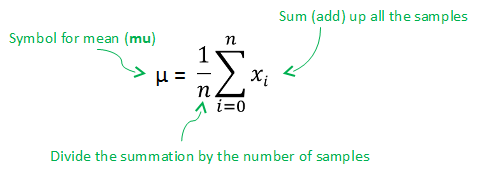
\includegraphics[width=4.9689in,height=1.7602in]{./media/Pictures/10000201000001DD000000A9D04A9B5021087E80.png}

In the above, the summation {} portion of the equation is read as
follows: for a set denoted by \emph{x} of size \emph{n}, we add (sum) up
each instance within \emph{x} between 1 and \emph{n}, denoted by
\emph{x}\textsubscript{\emph{i}}\emph{.}

For example, if we had seven values in a set, we add up (summation) the
seven values and then divide by seven, such as in the example below:

\textbf{ Samples = \{ 1, 2, 2.5, 2.5, 3, 3, 3.5 \}}

\textbf{ 1 + 2 + 2.5 + 2.5 + 3 + 3 + 3.5\\

-\/-\/-\/-\/-\/-\/-\/-\/-\/-\/-\/-\/-\/-\/-\/-\/-\/-\/-\/-\/-\/-\/-\/-\/-\/-\/-\/-\/-\/-\/-\/-\/-\/-\/-\/-\/-\/-
= 2.5 (}\emph{\textbf{µ}}\textbf{)\\
 7}

When referring to a sampling distribution (i.e., random subset of a
population distribution), the mean is denoted by the symbol \emph{x̅}
(x-bar).

The \emph{median }is the midpoint in a sorted distribution, such as a
population or sampling distribution. The \emph{median} is denoted by the
symbol\emph{ x̃ }(x-tilde). If the number of elements in the set is odd,
then the \emph{median} will be the midpoint (center) of the sorted set.
Below is an example:\\

\begin{quote}
\textbf{Sorted Set of Seven Samples = \{ 1, 2, 2.5, 2.5, 3, 3, 3.5 \}}
\end{quote}

\begin{quote}
\textbf{midpoint = 2.5 (}\emph{\textbf{x̃}}\textbf{)\\
}
\end{quote}

If the number of elements in the set is even, then the median is the
average of the two samples in the midpoint (center) of the sorted set.
Below is an example:

\textbf{Sorted Set of Eight Samples = \{ 1, 2, 2.5, 2.5, 3, 3, 3.5, 4
\}}

\begin{quote}
\textbf{midpoints = (2.5 + 3)/2 = 2.75 (}\emph{\textbf{x̃}}\textbf{)}
\end{quote}

\begin{quote}
\end{quote}

The \emph{mode} is the value in a set that occurs the most frequently.
For example, when plotting a bar chart, the tallest bar would be the
\emph{mode}. The mode is interpreted differently whether the values are
\emph{discrete} or \emph{continuous}. In the case of \emph{discrete}, it
is the value that occurs with the most frequency. For example, if the
values are a person's age in whole numbers, then the age that occurs the
most frequently is the mode, as in the example below:

\textbf{Sorted Set of Samples = \{ 20, 21, 21, 32, 32, 32, 36, 37, 37,
40 \}}

\textbf{mode = 32}

If the values are\emph{ continuous}, it is the range that occurs the
most frequently, where we group values into bins. For example of wealth,
one might group wealth into bins of \textless{}\$1K, \textless{}\$10K,
\textless{}\$100K, \textless{}\$250K, \textgreater{}\$1M. The bin with
the highest frequency would be the \emph{mode}.

\protect\hypertarget{anchor-13}{}{}\textbf{Standard Deviation}

The \emph{standard deviation} is a measurement to quantify the amount of
variation, also called dispersion, in a population or sampling
distribution. The \emph{standard deviation} for a population
distribution is denoted by the greek symbol {}(sigma) or
\emph{σ}\textsubscript{\emph{x.} }For a sampling distribution it is
denoted by the latin letter \emph{s}. The equation for calculating the
\emph{standard deviation} {}\emph{ }is denoted as:

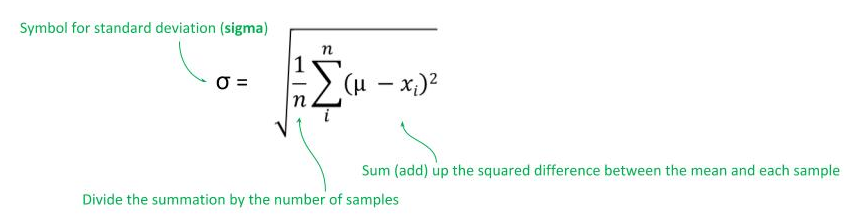
\includegraphics[width=6.5in,height=1.6945in]{./media/Pictures/1000000000000356000000DF329B9EE416FA68DB.png}

In the above, the summation {} portion of the equation is read as
follows:

\begin{enumerate}
\def\labelenumi{\arabic{enumi}.}
\item
  \begin{quote}
  Calculate the mean \emph{µ}.
  \end{quote}
\item
  \begin{quote}
  For a set denoted by \emph{x} of size \emph{n}, add (sum) up the
  square of the difference between each instance
  \emph{x}\textsubscript{\emph{i }}in the set \emph{x }from the mean of
  the set \emph{x} ( (\emph{µ} - x\textsubscript{i})\textsuperscript{2
  }).
  \end{quote}
\item
  \begin{quote}
  Then divide the summation by the number of instances (examples), and
  then take the square root of the result.
  \end{quote}
\end{enumerate}

Below is an example computation of the \emph{standard deviation}:

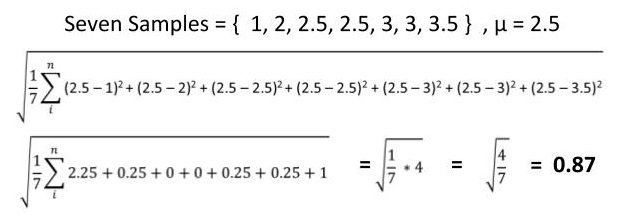
\includegraphics[width=5.2756in,height=1.9063in]{./media/Pictures/100000000000026C000000E06A81FDA5560DCB71.png}

\protect\hypertarget{anchor-14}{}{}\textbf{Normal Distribution}

A \emph{normal distribution}, also known as a Guassian distribution, is
a distribution used in propabilities for the expected random
distribution of samples within a population. The distribution is based
on observations of variability in the natural world of naturally
occurring things, such as shoe sizes, eye color, height, etc. In a
\emph{normal distribution}, we expect samples to be:

\begin{itemize}
\tightlist
\item
  68.2\% of the samples should be within one standard deviation of the
  mean.
\item
  95.4\% of the samples should be within two standard deviations of the
  mean.
\item
  99.8\% of the samples should be within three standard deviations of
  the mean.
\end{itemize}

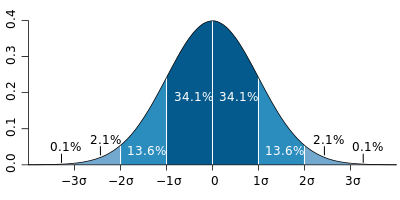
\includegraphics[width=4.1665in,height=2.0835in]{./media/Pictures/1000020100000190000000C8877241B1AADEA8F2.png}\\
Normal Distribution -
\href{https://commons.wikimedia.org/wiki/File:Standard_deviation_diagram.svg}{\emph{License}}

So what does this mean? It's interpreted as follows, if we could measure
every instance (sample) within a population of something naturally
occurring, we expect that 34.1\% of them to be less than the \emph{mean}
(average) value within one \emph{standard deviation} and conversely
34.1\% to be greater than the \emph{mean} within one \emph{standard
deviation}. And likewise for the second and third standard deviation.

Let's say our population was a bird specifies consisting of 1000 samples
and that the average weight (\emph{mean}) of the 1000 birds is 500 grams
with a \emph{standard deviation} of 100 grams. We would then expect that
68.2\% of the birds have their weight within the range of 400 to 600
grams, and expect 95.4\% to have their weights in the range 300 to 700
grams, and finally 99.8\% of the birds to have their weights in the
range 200 to 800 grams.

\protect\hypertarget{anchor-15}{}{}\textbf{Population vs. Sample}

Let's now cover the difference between a population and a sample. A
population is all the instances of something we are measuring, such as
all male shoe sizes in North America. If one had the entire enumeration
of male shoe sizes in North America, we would refer to that enumeration
as a population. Given a population, we can define parameters for it,
such as the \emph{mean}, \emph{standard deviation} and \emph{size}, as
depicted below. These values are not statistical since the actual values
are known by enumeration of the entire population.

In most cases, we don't have the ability to measure an enumeration of an
entire population. Instead, we take samples, where a sample consists of
some plurality of instances within the population. From that sample we
calculate the probability of it being representative of the population,
if the population was known. This is what is meant by a statistic.

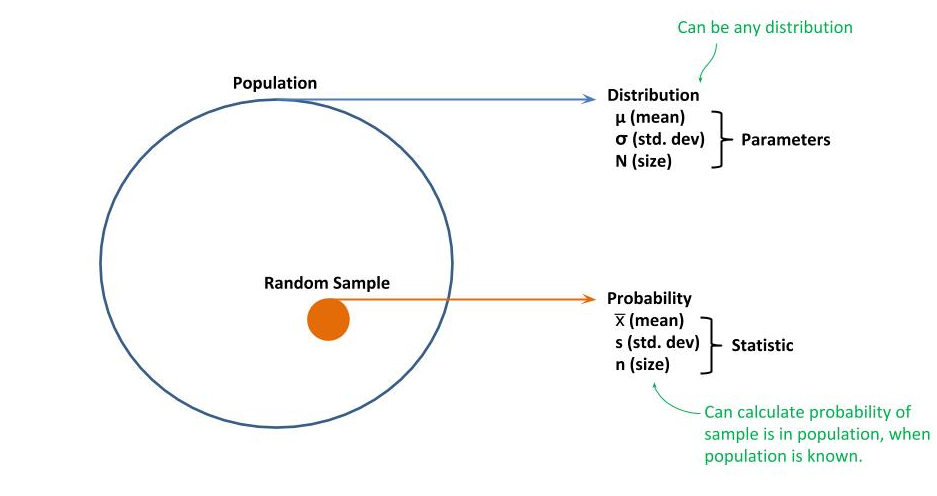
\includegraphics[width=6.5in,height=3.4445in]{./media/Pictures/10000000000003A9000001F0AD9A8C86E9DA02A2.png}\\
~\\

\protect\hypertarget{anchor-16}{}{}\textbf{Sampling Distribution}

So far, we have described a population and a sample within a population.
If we now take a random set of samples, also referred to as a draw, from
the population, those random samples form a \emph{sampling
distribution}. As more samples are drawn at random, the sampling
distribution will exhibit more of the characteristics of the population.

While there is no predetermined way to know with certainty on how many
random samples to draw to be representative of the population, it is a
common practice to set that threshold at 30 samples chosen at random.
For example, if I polled 30 people at random within a voting district on
who they would vote for, it is likely the \emph{sampling distribution
}would be representative of the actual distribution within the voting
district.

If we calculate the mean of each sample, denoted by the symbol \emph{x̅},
as a set and then calculated the mean of the set of sample means,
denoted by the symbol \emph{µ}\textsubscript{\emph{x̅} }, we expect the
sample means to approximate that of the population mean \emph{µ }:

\emph{µ}\textsubscript{\emph{x̅ }}\emph{= µ}

If we calculate the standard deviation for the set of sampling means,
denoted by the symbol {}\textsubscript{\emph{x̅} }, we expect the
standard deviation of the sample means to approximate the standard
deviation of the population divided by the square root of the size
(number of instances) of a sample: {}\textsubscript{\emph{x̅} } =
{}\emph{ / }{}

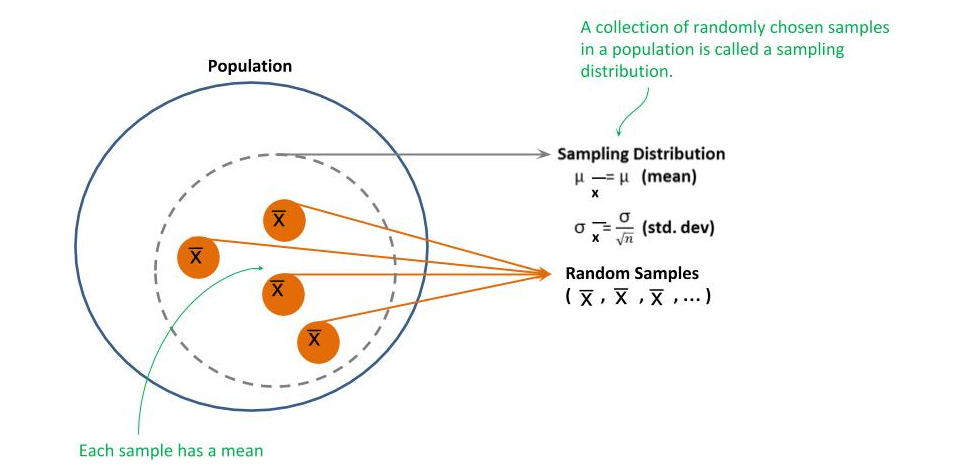
\includegraphics[width=6.5in,height=3.1528in]{./media/Pictures/10000000000003C0000001D195E8748D92D25AA8.png}\\

\protect\hypertarget{anchor-17}{}{}\textbf{Central Limit Theorem}

You might question that all natural occurring events follow this
distribution. Yes, there are many factors that could result in a
distribution other than the \emph{normal distribution}. But even in
those distributions, if one draws random samples from the population and
plot the mean of each sample, that the plots of the sample means will
follow a \emph{normal distribution}. This is known as the \emph{central
limit theorem}. This can then be used to approximate what is the
\emph{population mean} and \emph{standard deviation}, without having
enumerated the entire population.

Typically, the first sample means one plots, one will not yet see a
normal (Gaussian) distribution. But as more samples are drawn and the
sample means plotted, the plot will gradually form a \emph{normal
distribution}, as depicted below:

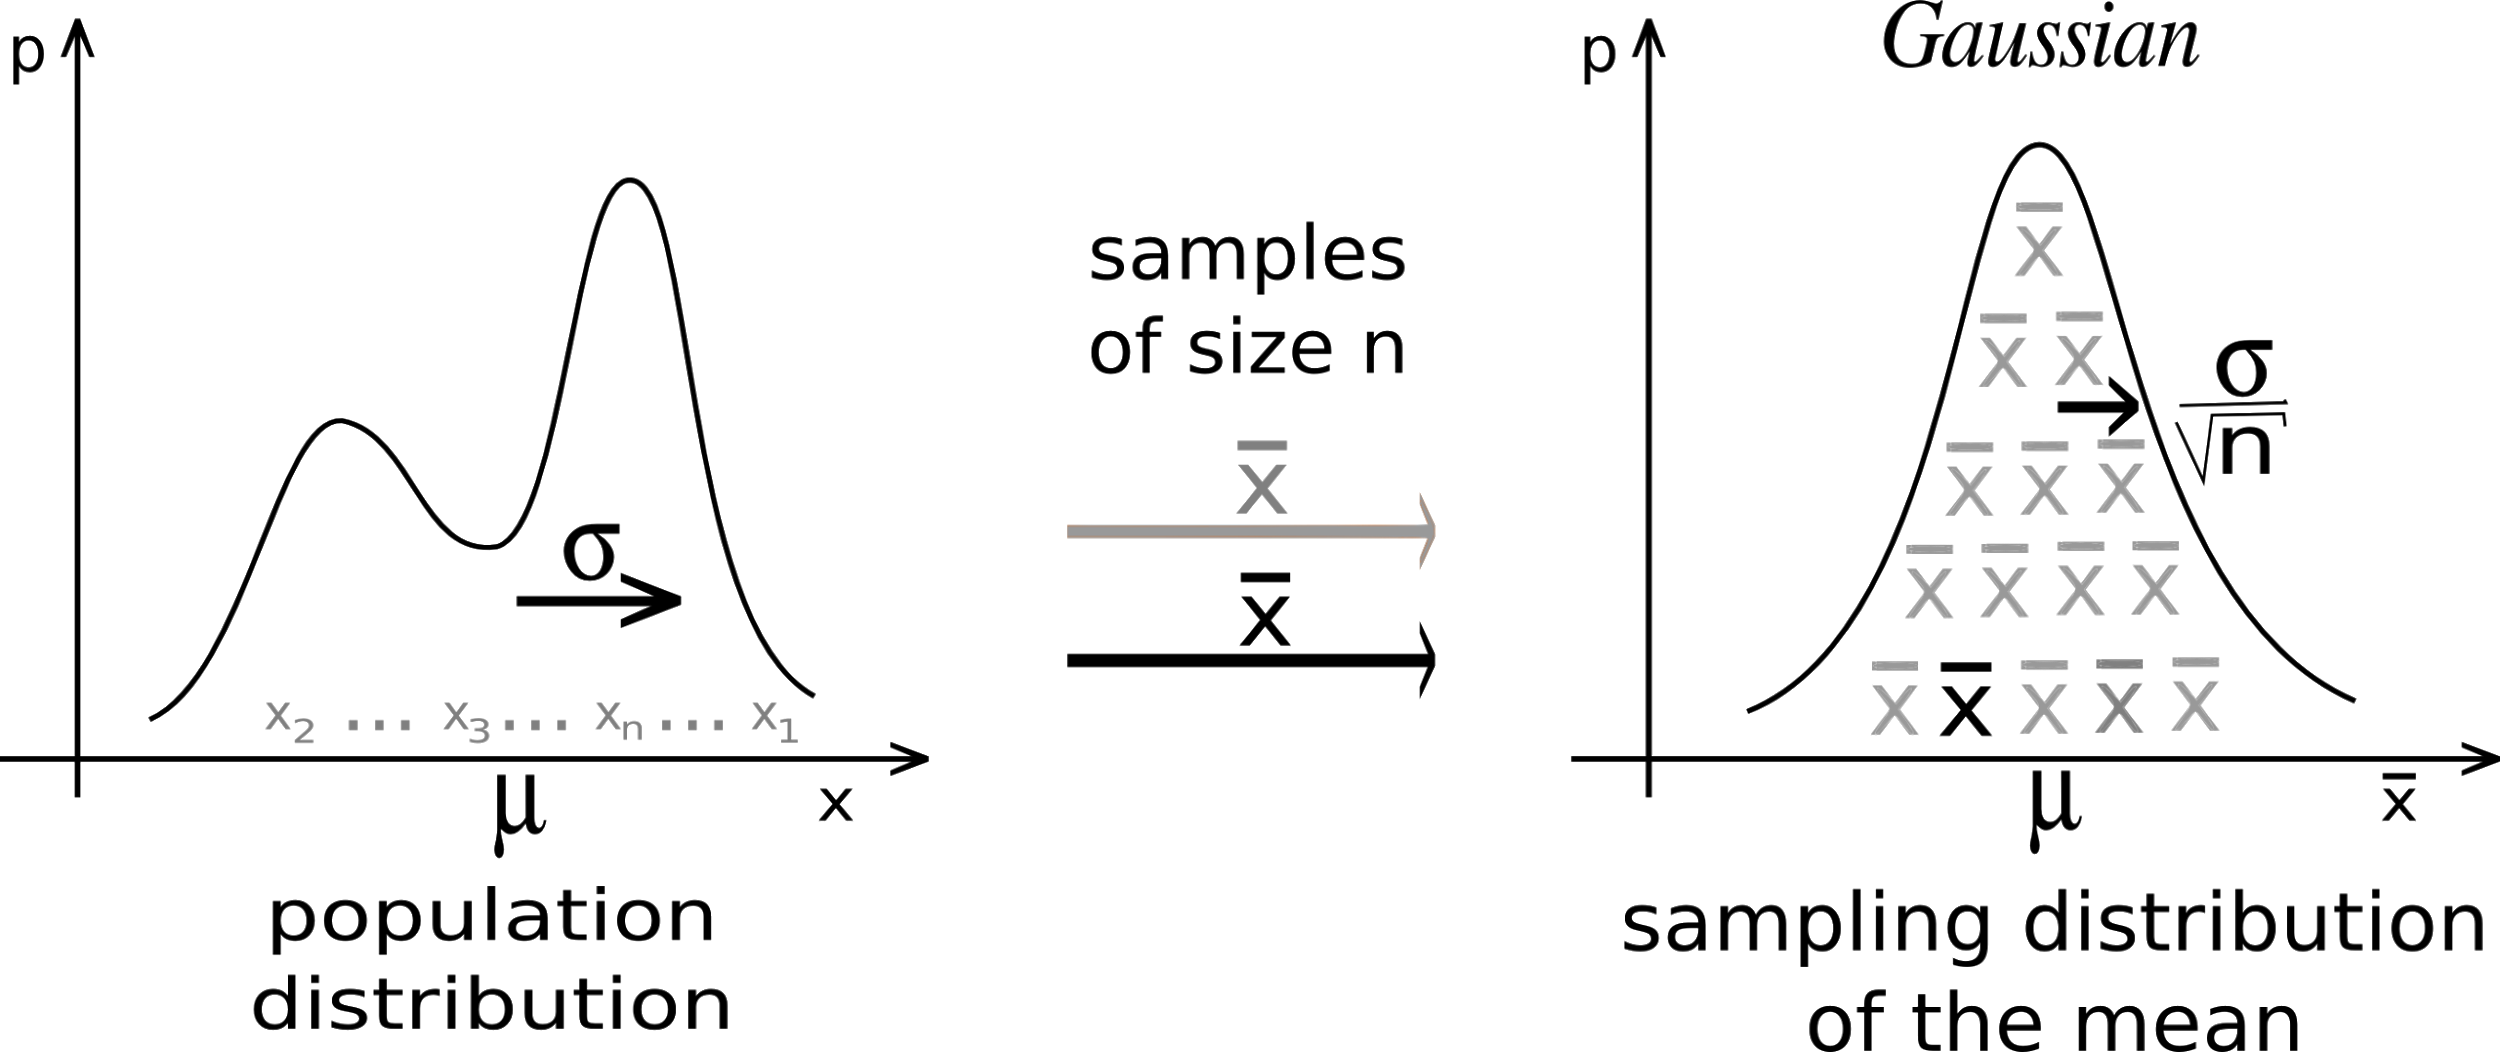
\includegraphics[width=6.5in,height=2.7362in]{./media/Pictures/10000201000009C40000041CEF1CE226046F1496.png}

\textbf{}Central Limit Theorem -
\href{https://en.wikipedia.org/wiki/Central_limit_theorem\#/media/File:IllustrationCentralTheorem.png}{\emph{License}}

\textbf{Z-Score}

\textbf{\\
}The term \emph{Z-score} is used in statistics to measure how far a
sample or instance is from the population \emph{mean}.\emph{ Z-score}
are equal to \emph{standard deviations}. Thus a \emph{Z-score} of 1 is
the same as one \emph{standard deviation} from the \emph{mean}.

Z-scores are used in statistics to calculate the probability of an
instance occurring within a normal distribution. It also provides a
method for comparing scores from different distributions. For example,
assume a student has scored 70\% and 80\% on two different tests. Since
the two tests are different distributions in results, knowing the
percentages does not tell us how the student did across the two tests.

Instead, we determine the student's \emph{Z-score} for each test based
on the distribution of results for each test. Using our example above,
if the \emph{Z-score} on the first test was 1 and on the second test was
0.9, one could say that the student did worse on the second test, even
though the percentage was higher. Using \emph{Z-scores} provides a
method to normalize the results between different distributions for
comparison.

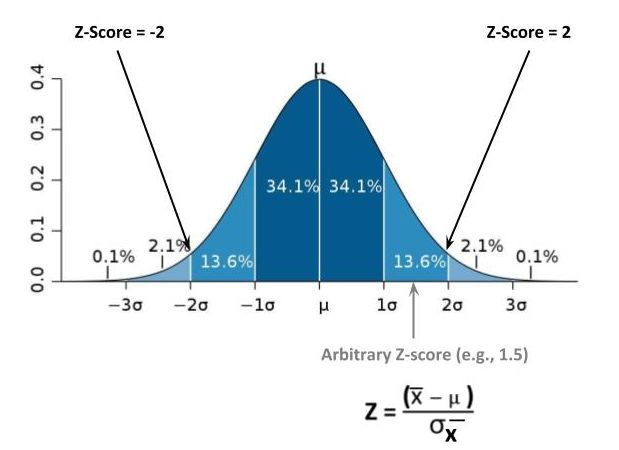
\includegraphics[width=4.1819in,height=3.0402in]{./media/Pictures/100002010000026B000001C2EEC0FB4C6946A73E.png}\textbackslash{}

\textbf{Standard Normal Probabilities Table}

The standard normal probability tells you the probability that a
\emph{Z-score} falls within an area of the normal distribution. These
probabilities can be looked up in the
\href{http://ux1.eiu.edu/~aalvarado2/z_table.pdf}{Standard Normal
Probabilities Table}.

Using a student's test score as an example, if there \emph{Z-score} for
the test was -1.0, then using the table we find that 15.87\% of the
students scored the same or less on the test. If the \emph{Z-score} was
1.0, we find that 84.13\% of the students scored the same or less; or in
other words the student scored in the 84 percentile.

\textbf{\\
An Example - Robotic ForkLift}

Let's demonstrate how to use all the terms and equations we've
discussed. In our example, we will calculate the probability of a
robotic forklift picking up a pallet of unknown weight without tipping
over. Let's assume the following are the known facts:

\begin{itemize}
\tightlist
\item
  Warehouse: The historical data for boxes in the warehouse
  (\emph{population}) is a \emph{mean} weight of 50 lbs and a
  \emph{standard deviation} of 10 lbs.
\item
  Robotic Forklift: Has a weight lifting limit of 560 lbs.
\end{itemize}

Let's assume the following scenario:

\begin{itemize}
\tightlist
\item
  Pallet of Boxes: We have a pallet of ten boxes of unknown weights.
\item
  Question: What is the probability that the robotic forklift can lift
  the pallet?
\end{itemize}

Let's do some initial calculations. We know the \emph{population mean}
is 50 lbs. We know that given sufficient random samples in a
\emph{sampling distribution}, the \emph{mean} across random samples of
ten pallets should be the same as the population mean.

\emph{µ}\textsubscript{\emph{ (population) }}\emph{ =
10}\textsubscript{\emph{\\
}}\emph{µ}\textsubscript{\emph{x̅ }}\emph{ = µ}\textsubscript{\emph{
}}\emph{ = 10}

We also know that the standard deviation for our random samples will be
the\emph{ standard deviatio}n of the population (warehouse) divided by
the size of our random sample:

{}\textsubscript{\emph{ (population) }}\emph{= 10\\
}{}\textsubscript{\emph{x̅} } = {}\emph{ / }{}\emph{ = 10 / }{}\emph{ =
3.16}

Next we calculate the\emph{ maximum mean} for a random sample (pallet of
ten boxes), denoted by the symbol \emph{x̅}\textsubscript{\emph{max}}. We
know that the maximum weight the robotic forklift can lift is 560 lbs.
Given that our pallet size is ten boxes, then the maximum mean will be
the maximum weight (560 lbs) divided by the size of the pallet (10
boxes):

\emph{X̅}\textsubscript{\emph{max}}\emph{ = 560 / 10 = 56}

Next, we calculate a Z-score so we can determine the probability that
this pallet of unknown weight can be lifted by the robotic forklift. We
use the above computations to calculate the \emph{Z-score }for the
probability that a pallet of ten boxes of unknown weight will be a
maximum of 560 lbs. Using the equation for a \emph{Z-score}, we get the
difference between the \emph{maximum mean} (56 lbs) and the
\emph{population mean }(6 lbs) and divide it by the \emph{sampling
standard deviation} (3.16), which gives a \emph{Z-score} of 1.9.

\begin{quote}
\emph{Z = ( X̅}\textsubscript{\emph{max}}\emph{ - µ ) /
}{}\textsubscript{\emph{x̅ }}\emph{ = (56 - 50) / 3.16 = 1.9}
\end{quote}

We now look up the \emph{Z-score} of 1.9 in the Standard Normal
Probabilities Table, which gives a probability of 97.13\% likelihood
that this pallet of ten boxes of unknown weight can be lifted by the
robotic forklift.

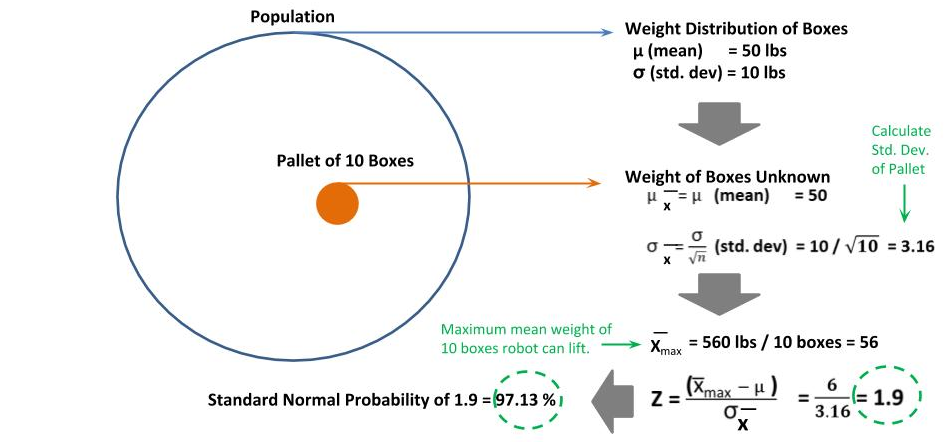
\includegraphics[width=6.5in,height=3.0417in]{./media/Pictures/10000201000003B2000001BABCFD9AAF5929DA03.png}

\textbf{Null Hypothesis}

Another basic methodology in statistics is the \emph{null hypothesis}.
This methodology is used when one has a hypothesis, but can't directly
prove it. So instead, one determines the opposite of the hypothesis
(i.e., would be true if hypothesis is false), referred to as the
\emph{null hypothesis}, and then proves instead that the \emph{null
hypothesis} is false within a statistical level of confidence. The
\emph{null hypothesis} to disprove and the hypothesis to prove are
denoted by H\textsubscript{0} and H\textsubscript{1}, respectively.

Let's use as an example of a population which is the transaction history
for a store. Let's assume we have the following known facts, that the
\emph{population mean} for a transaction is \$25 with a\emph{ standard
deviation} of \$5.

\emph{µ}\textsubscript{\emph{ (population) }}\emph{ = \$25\\
}{}\textsubscript{\emph{ (population) }}\emph{= 10}

Let's assume a new set of transactions, such as all the transactions for
today, which will be our transaction sample, and that the
transaction\emph{ sample mean} is \$26.50.

\emph{X̅}\textsubscript{\emph{ }\emph{(sample) }}\emph{= \$26.50}

Let's define the hypothesis H\textsubscript{1} (what we want to prove)
and the opposite, the \emph{null hypothesis} H\textsubscript{0}:

\begin{itemize}
\tightlist
\item
  H\textsubscript{0}: The mean price of a transaction has increased
  (\emph{µ} \textgreater{} \$25)
\item
  H\textsubscript{1}: The mean price of a transaction has not increased
  (\emph{µ} {} \$25)
\end{itemize}

In other words, we will prove that nothing (the mean) has changed by
disproving that the \emph{population mean} has increased within a
significant level of confidence. In this example, we assume an average
size (n) of a transaction is 10 items. First, we calculate the
\emph{sample standard deviation}:

{}\textsubscript{\emph{ (population) }}\emph{= 5\\
}{}\textsubscript{\emph{x̅} } = {}\emph{ / }{}\emph{ = 5 / }{}\emph{ =
1.58}

Next, we calculate the \emph{Z-score} and then look it up in the
Standard Normal Probabilities Table:

\begin{quote}
\emph{Z = ( X̅ - µ ) / }{}\textsubscript{\emph{x̅ }}\emph{ = (26.5 - 25) /
1.58 = 0.95}
\end{quote}

\begin{quote}
\emph{Standard Normal Probability for 0.95 is 82.18\%}
\end{quote}

We interpret the above probability that there is a 82.18\% likelihood
that this sample is within the existing\emph{ population}. In other
words, we have a 82.18\% confidence that the\emph{ population mean}
(transaction mean) has not gone up, and only a 17.82\% that it has.

Let's now show the effect of the sample size. We will use the same
example, except now we assume an average size (n) of a transaction is
100 items. We calculate the \emph{sample standard deviation}:

{}\textsubscript{\emph{ (population) }}\emph{= 5\\
}{}\textsubscript{\emph{x̅} } = {}\emph{ / }{}\emph{ = 5 / }{}\emph{ =
0.5}

Now we calculate the \emph{Z-score} and then look it up in the Standard
Normal Probabilities Table:

\begin{quote}
\emph{Z = ( X̅ - µ ) / }{}\textsubscript{\emph{x̅ }}\emph{ = (26.5 - 25) /
0.5 = 3}
\end{quote}

\begin{quote}
\emph{Standard Normal Probability for 3 is 99.97\%}
\end{quote}

At a transaction sample size of 100, we would have the probability
(confidence) of 99.97\% that the sample is within the \emph{existing
population}, and that the \emph{population mean} has not increased.

\textbf{ArgMax \& SoftMax}

The \emph{argmax }and \emph{softmax} functions appear frequently in
statistics and deep learning. First, let's define what the
\emph{max}(\emph{x}\textsubscript{\emph{1}}\emph{ ..
x}\textsubscript{\emph{n}}\emph{ }{}\emph{ x}) function is. It's a
function, given some set of values \emph{x}, consisting of elements
\emph{x}\textsubscript{\emph{1}} to\emph{ x}\textsubscript{\emph{n}}, it
returns the element x\textsubscript{j} which is the largest value of all
the elements.

One can define the\emph{ max} function as being the condition where the
instance \emph{x}\textsubscript{\emph{j}} is greater than or equal to
all other instances in the set \emph{x}, which can be described as the
equation:\\

\emph{x}\textsubscript{\emph{j}}\emph{ ≥
x}\textsubscript{\emph{i}}\emph{ , x ∈ S}

Let's cover some of the symbols we use here to describe the \emph{max
}function:\\
~\\
S : Set of discrete values.

∈ : Symbol for an element of a set.

x\textsubscript{i } : An Instance of an element of a set.

\textsubscript{}≥ : Greater than or equal to for all elements in a set.

\emph{\textbf{ArgMax}}

The \emph{argmax} function instead returns a value
\emph{x}\textsubscript{\emph{i}} from a set \emph{x}, which maximizes
the result of a function, denoted by \emph{f(x)}.The \emph{argmax} takes
as arguments the function and the set of values, which is represented
as:

\emph{argmax(f(x}\textsubscript{\emph{1}}\emph{ ..
x}\textsubscript{\emph{n}}\emph{ }{}\emph{ x))}

The condition is met when the output of the function\emph{ f(x)} for at
least one instance \emph{x}\textsubscript{\emph{j}} is greater than or
equal to all outputs for \emph{x }{}\emph{ S}. This equation can be
expressed as:

\emph{f(xj}\textsubscript{\emph{)}}\emph{ }{}\emph{
f(x}\textsubscript{\emph{i}}\emph{), x }{}\emph{ S}

Let's explain this equation. There is some instance x\textsubscript{j}
within all elements of the set \emph{S} that is greater than or equal to
all other instances x\textsubscript{i}.

For an example, let's assume of f(x) is the function \emph{x*(x-10)},
which can be expressed as:

\emph{f(x) = x *(x-10)}

Below is the evaluation of the function for discrete integer numbers
between 0 and 10:

\emph{f(x = 0) = 0 * (10 - 0) = 0\\
f(x = 1) = 1 * (10 - 1) = 9\\
f(x = 2) = 2 * (10 - 2) = 16\\
f(x = 3) = 3 * (10 - 3) = 21\\
f(x = 4) = 4 * (10 - 4) = 24\\
f(x = 5) = 5 * (10 -5 ) = 25← maximizes the function\\
f(x = 6) = 6 * (10 - 6 ) = 24\\
f(x = 7) = 7 * (10 - 7) = 21\\
f(x = 8) = 8 * (10 -8) = 16\\
f(x = 9) = 9 * (10 - 9) = 9\\
f(x = 10) = 10 * (10 -10) = 0}

In the above example, the value 5 maximizes the result of the function.
Thus, argmax( x * (x-10) ) is 5.

\emph{\textbf{SoftMax}}

The \emph{softmax} function, also referred to as a boltzmann function in
physics, is used when predicting a probability distribution, such as in
classification (e.g., type of fruit) and each predict makes an
independent prediction. For simplicity image you have three algorithms,
one predicts if something is an apple, another a pear, and the other a
peach, as depicted below.

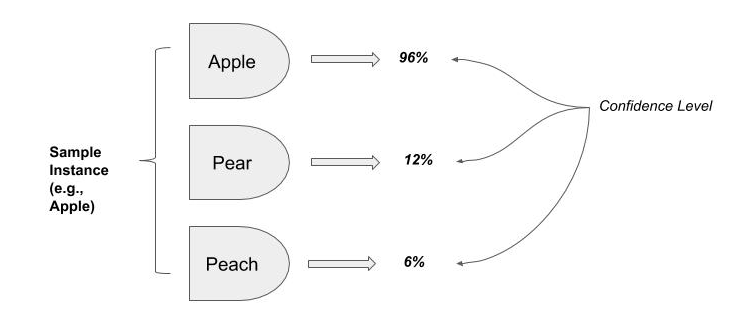
\includegraphics[width=6.5in,height=2.75in]{./media/Pictures/10000201000002EE0000013EA8B9E59EF9EF2AEC.png}

The above example, since each prediction (percent confidence level) is
independent, that there is no reason to expect the sum of all the
predictions to add up to 100\%. That's a problem when in statistics when
each prediction is independent of the other. This problem is solved
using the \emph{softmax} function. The \emph{softmax} function takes a
set of any real values and squashes them into a normalized probability
distribution that will sum up to one.

In neural networks which perform classification, each output node from
the neural network makes an independent prediction of the associated
class. Since each prediction is independent, all the output predictions
are passed through a \emph{softmax} function, such that the resulting
set of predictions sums up to one (i.e., 100\%), as depicted below:

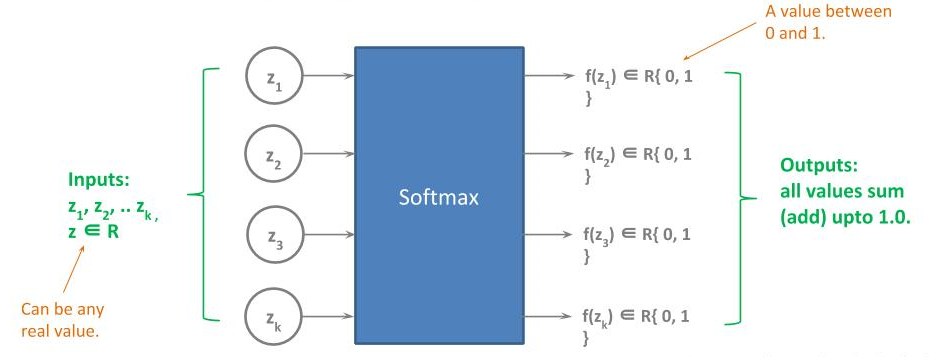
\includegraphics[width=5.7563in,height=2.2165in]{./media/Pictures/10000201000003A1000001659050BFE773D054A7.png}

Below is the equation for a \emph{softmax} function:

\begin{quote}
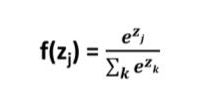
\includegraphics[width=2.0835in,height=1.0209in]{./media/Pictures/10000201000000C800000062DD85CFB4A3F8D9C2.png}
\end{quote}

Let's cover some of the symbols we use here to describe the
\emph{softmax} function:\\
~\\
R : Set of real values.

∈ : Symbol for an element of a set.

z : The set of input values.

z\textsubscript{j} : An instance in the set of input values.\\
k : The number of inputs.

e : The natural number, also known as Euler's number (2.718\ldots{})

Below is an example of applying the softmax function to the input set
\{8, 4, 2\}:\\
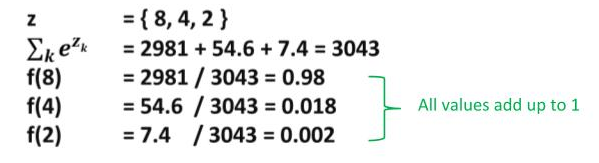
\includegraphics[width=6.2398in,height=1.698in]{./media/Pictures/1000020100000257000000A38EF7D3F5CA73F89B.png}

\textbf{Next}

In the next part we will cover the fundamental principles of linear and
logistic regression.

\protect\hypertarget{anchor-18}{}{}

\protect\hypertarget{anchor-19}{}{}\textbf{Part B - Linear/Logistic
Regression}

In this part, we will start by covering the most fundamental model in
traditional machine learning, a \emph{simple linear regression}, and
then advance to \emph{multiple linear regression,} \emph{logistic
regression} and the principles behind feature engineering.

\textbf{Simple Linear Regression}

A \emph{linear regression} is a method to predict a correlation between
one or more independent variables, also referred to as features, and a
dependent variable, also referred to as the label. A \emph{linear
regression} performs well when there is a strong linear relationship
between the independent variables and the dependent variable.

In a \emph{simple linear regression}, we have one independent variable
(feature) and one dependent variable (label). As an example of a simple
linear regression would be to model how speeding is correlated with
traffic deaths.

If the independent variable is highly correlated with the dependent
variable, it will appear as a (near) straight line relationship when
plotted.

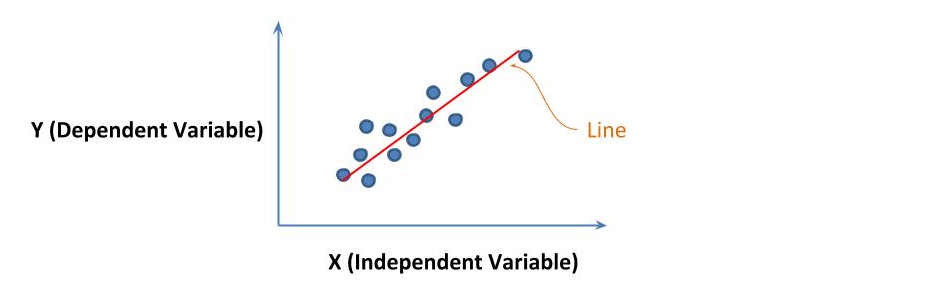
\includegraphics[width=6.5in,height=1.9445in]{./media/Pictures/10000000000003B10000011B0270CDF0249E3ACD.png}

In a simple \emph{linear regression}, one finds a linear approximate
relationship (line) relationship between the independent and dependant
variables. In machine learning, the independent variable is commonly
referred to as a feature and denoted by \emph{x}, and the dependent
variable is commonly referred to as the label and denoted by \emph{y}.

It's likely you are already familiar with a \emph{simple linear
regression} from high school or college math, and is known by several
names. We will cover several example representations next.

In elementary geometry, a \emph{simple linear regression} is the same as
the definition of a line, which is represented by the equation:

\emph{y = mx + b}

y : dependent variable\\
x : independent variable\\
m : slope of the line\\
b : y-intercept

In the above, the slope (m) is a coefficient which determines the angle
of the line when plotted on a 2D graph. The y-intercept (b) is the value
on the y axis that the line crosses.

In linear algebra, a \emph{simple linear regression} is represented by
the equation:

\emph{y = a + bx}

y : dependent variable\\
x : independent variable\\
a: y-intercept\\
b: coefficient (i.e., slope)

In machine learning, a \emph{simple linear regression} is represented by
the equation:

\emph{y = b}\textsubscript{\emph{ }}\emph{+
w}\textsubscript{\emph{1}}\emph{x}\textsubscript{\emph{1}}

y : dependent variable\\
x\textsubscript{1 }: independent variable\\
b\textsubscript{ }: bias (i.e., y-intercept)\\
w\textsubscript{1} : weight (i.e., slope)

In linear algebra method, we have a set of x values (i.e., data) where
we plot each value on a x-axis/y-axis 2D graph, which is referred to as
a scatter plot. We then attempt to find the best fitting line through
the plotted points, as depicted below:

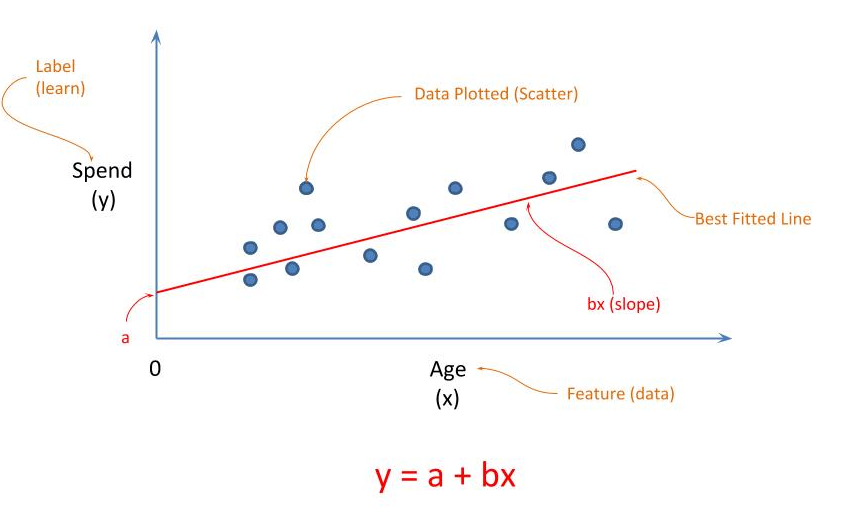
\includegraphics[width=4.9634in,height=2.9661in]{./media/Pictures/100000000000034E000001FDDE39AA80C8713DAF.png}

What is meant by best fitted line, is a line that can be drawn through
the plotted points that has the least amount of accumulated error
between the actual plot point (\emph{y}) and the point predicted by the
line, commonly referred to as \emph{ŷ} (y-hat).

This accumulated error is referred to as a \emph{cost function}. In a
\emph{cost function}, one uses a function to calculate the difference
between the actual points (\emph{y}) and the predicted points
(\emph{ŷ}), commonly referred to as a \emph{loss function}. A summation
of the losses is then done and divided by the number of points. The
objective of fitting the best line is to minimize the resulting value of
the \emph{cost function}. In other words, the best fitting line is the
line that results in the least value of the \emph{cost function}.

In a \emph{simple linear regression}, the common practice for a
\emph{loss function} is the \emph{mean square error }(mse) method. In
the\emph{ mean square error }method, we sum up the squared difference
between the actual and predicted points \emph{(y -
ŷ)}\textsuperscript{\emph{2}} and then divide by the number of points.

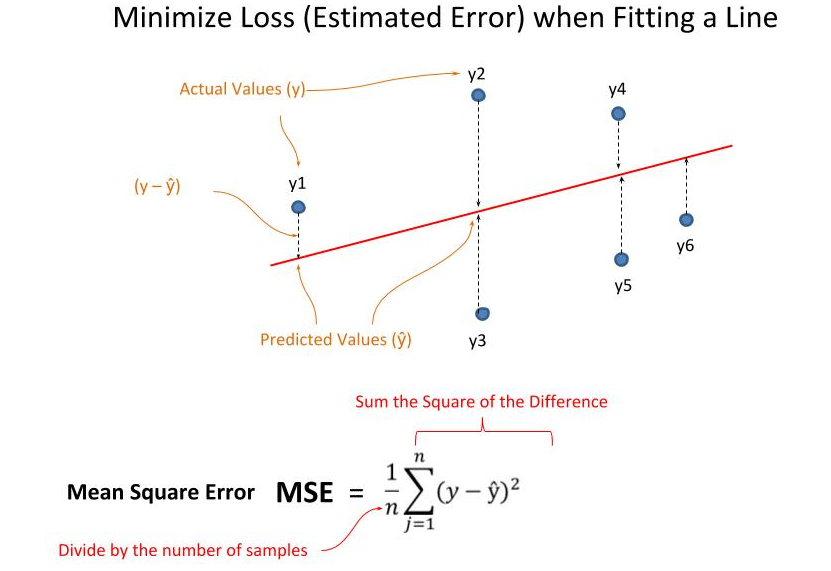
\includegraphics[width=5.6307in,height=3.8709in]{./media/Pictures/100000000000033F0000023B582285DC694927AE.png}

Why would we square the difference? The purpose of squaring the
difference is that it penalizes points that are farther away from the
predicted points, as well as making error always a positive value.

The solution to a \emph{simple linear regression} for a \emph{mean
square error loss function} can be factored and computed as:

\begin{quote}
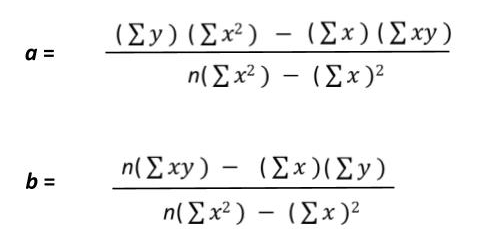
\includegraphics[width=2.7756in,height=1.3791in]{./media/Pictures/10000000000001DF000000EF6EC832592B6C2120.png}
\end{quote}

\begin{quote}
{} : sum of all values of \emph{x}.\\
{} : sum of all values of \emph{y}.\\
{} : sum of all values x * y.\\
{} \emph{x}\textsuperscript{\emph{2}} : sum of all values
\emph{x}\textsuperscript{\emph{2}}.
\end{quote}

Other common \emph{loss functions} used in a \emph{linear regression}
are the \emph{mean absolute error} (mae) and \emph{root mean square
error }(rmse). In the \emph{mean absolute error}, the summation is
absolute difference between the actual value and predicted value, which
as in mse, always results in a positive error value.

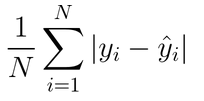
\includegraphics[width=1.4693in,height=0.728in]{./media/Pictures/10000000000000CC000000656A248F87FE9192E0.png}

In the \emph{root mean square error}, we take the square root of the
\emph{mean square error}.

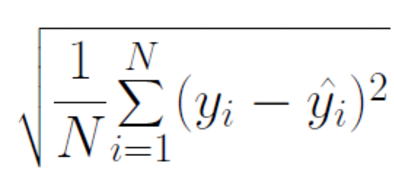
\includegraphics[width=1.6075in,height=0.7799in]{./media/Pictures/100000000000018A000000BF672A53832F8D4740.png}

The reason one calls the variable we are predicting the dependent
variable, is that the value of the dependent variable is dependent on
the values of other (independent) variables, while the converse is not
true. Given the earlier example of using Age to predict Income. The
variable Income is the dependent variable because it's value is
dependent on Age. But conversely, the variable Age is an independent
variable because its value is not dependent on Income.\\

\textbf{Multiple Linear (Multivariate) Regression}

In a \emph{multiple linear regression}, we have two or more independent
variables (features) and one is finding a correlation between multiple
independent variables and the dependent variable (label), for example
how age and income correlates with spending. If there is (or near)
linear correlation, we expect that when the data is plotted on a graph,
there is a hyperplane relationship between the multiple independent
variables (features) and the dependent variable (label).

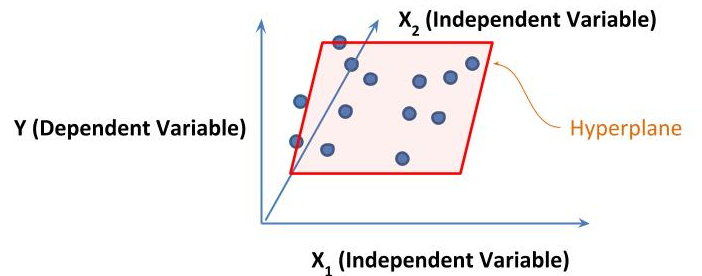
\includegraphics[width=3.8917in,height=1.5193in]{./media/Pictures/10000000000002BE000001142ECBF49DE460C98A.png}

In machine learning, a \emph{multiple linear regression} is represented
by the equation:

\emph{y = b}\textsubscript{\emph{ }}\emph{+
w}\textsubscript{\emph{1}}\emph{x}\textsubscript{\emph{1 }}\emph{+
w}\textsubscript{\emph{2}}\emph{x}\textsubscript{\emph{2 }}\emph{+
\ldots{} w}\textsubscript{\emph{n}}\emph{x}\textsubscript{\emph{n\\
}}~\\
w\textsubscript{1}, w\textsubscript{2}, \ldots{} w\textsubscript{n}:
weights for \emph{n} independent variables.\\
x\textsubscript{1}, x\textsubscript{2}, \ldots{} x\textsubscript{n :
}data for \emph{n} independent variables.

A \emph{multiple linear regression} is also referred to as a
\emph{multivariate regression}.

\textbf{Logistic Regression}

In \emph{logistic regression}, also referred to as a \emph{logistic
classifier}, is a regression whose result is a binary value (not a real
value). A \emph{logistic regression} is used when predicting if
something is true or false, such as whether someone would default on a
loan. A \emph{logistic regression} can also be used for a binary
classification (i.e., two classes), by reducing to predicting whether
one class is true or false; and if false then it's implied the other
class is true.

In a \emph{linear regression}, the dependent variable is always a
continuous value. That is, it's a real number vs. a discrete value. In a
\emph{logistic regression}, the dependent variable is a discrete value,
where a binary value is an example of a discrete value.

In machine learning, a \emph{logistic regression} is represented by the
equation:

\begin{quote}
\emph{log(}{}\emph{) = c}\textsubscript{\emph{ }}\emph{+
w}\textsubscript{\emph{1}}\emph{x}\textsubscript{\emph{1 }}\emph{+
w}\textsubscript{\emph{2}}\emph{x}\textsubscript{\emph{2 }}\emph{+
\ldots{} w}\textsubscript{\emph{n}}\emph{x}\textsubscript{\emph{n}}
\end{quote}

\begin{quote}
\emph{c }: the probability of \emph{y} being true independently of the
independent \\
 variables \emph{x}\textsubscript{\emph{1 }}\ldots{}
\emph{x}\textsubscript{\emph{n}}.\\
\emph{y} : the probability of \emph{y} being true.\\
1 - \emph{y} : the probability of \emph{y} not being true.
\end{quote}

Sometimes, one will see the above equation where a \emph{P} is used in
place of \emph{y}. It is common in statistics to denote the probability
of an event with the symbol \emph{P}.

\begin{quote}
\emph{log(}{}\emph{) = c}\textsubscript{\emph{ }}\emph{+
w}\textsubscript{\emph{1}}\emph{x}\textsubscript{\emph{1 }}\emph{+
w}\textsubscript{\emph{2}}\emph{x}\textsubscript{\emph{2 }}\emph{+
\ldots{} w}\textsubscript{\emph{n}}\emph{x}\textsubscript{\emph{n}}
\end{quote}

The symbol \emph{c }is a constant value that represents the portion of
the probability distribution that the event (\emph{Y}) could be true
independently of the values (existence) of the independent variables.
For an example, let's assume our dependent variable is to classify
whether an email is either spam or not spam. In this example, the
constant \emph{c} would be the portion of emails that are spam, but
could not be predicted by the independent variables.

The expressions \emph{Y} and \emph{1 - Y}, and conversely \emph{P} and
\emph{1 - P}, represent the probability of the event happening (true)
and not happening (false). Since probabilities is a percentage
represented in the range 0 to 1, then the probability of something not
being true is 1 minus the probability of being true, hence the term
\emph{1 - Y} (or \emph{1 - P}).

The expression\emph{ log( Y / (1 - Y) ) }when plotted for a continuous
range of values for \emph{Y} between 0 and 1 will be an S-curve between
0 and 1. When training using a \emph{logistic regression,} the objective
is to find the best fitting S-curve to the data, vs. best fitting line
in a \emph{linear regression}. There are numerous forms of S-curves in
statistics. Some common ones are the logistic function (shown below),
the error function, the sigmoid and the hyperbolic tangent.

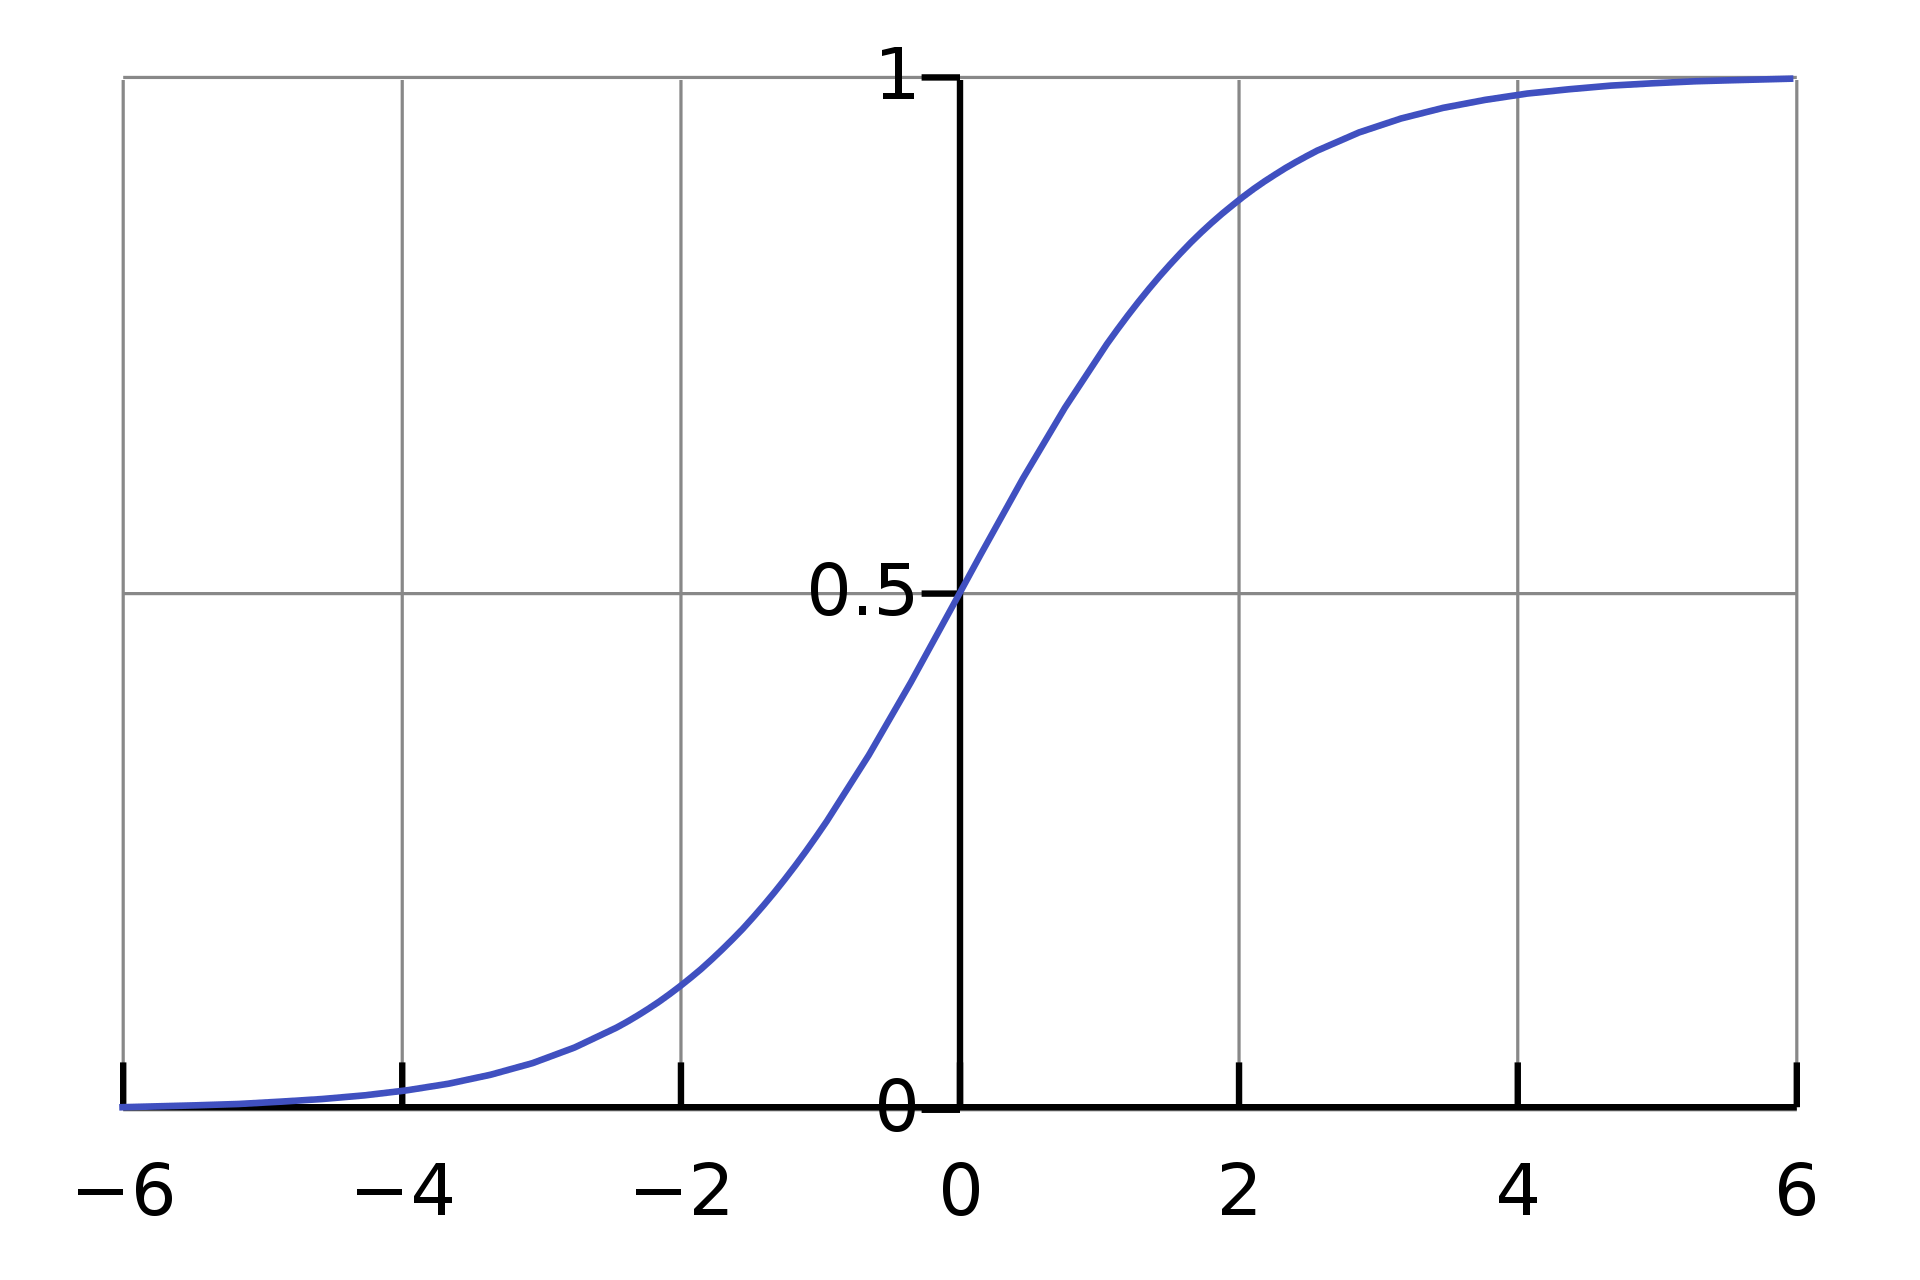
\includegraphics[width=2.661in,height=1.7764in]{./media/Pictures/100002010000078000000500E667F9F6C56BE3AE.png}\\
 Logistic Function (S-curve) -
\href{https://en.wikipedia.org/wiki/Logistic_function\#/media/File:Logistic-curve.svg}{\emph{License}}

Since we are fitting a S-curve, the cost function used to calculate the
error between the predicted \emph{ŷ }and actual y is the\emph{ log loss}
function, also referred to as cross entropy. The log loss function is
represented by the equation:

\emph{-(y * log}\textsubscript{\emph{e}}\emph{(ŷ) + (1 -
y)log}\textsubscript{\emph{e}}\emph{(1 - ŷ))}

log\textsubscript{e} : natural logarithm (also denoted by ln)\\
y : actual value (0 or 1)\\
\emph{ŷ } : predicted probability between 0 and 1.

The loss function for a logistic regression is the summation of the log
loss between the predicted and actual values, divided by the number of
values, as represented below:

\begin{quote}
{}{}\emph{-(y}\textsubscript{\emph{i }}\emph{*
log}\textsubscript{\emph{e}}\emph{(ŷ}\textsubscript{\emph{i}}\emph{) +
(1 -
y}\textsubscript{\emph{i}}\emph{)log}\textsubscript{\emph{e}}\emph{(1 -
ŷ}\textsubscript{\emph{i}}\emph{))}
\end{quote}

For prediction, one picks a threshold within the 0 to 1 range to predict
when the example is or is not true (e.g., spam or not spam). By default,
this would be 0.5. Values below 0.5 are considered false and values
above are considered true.

Once the logistic regression is trained, one may choose to slightly
modify the threshold value for prediction, based on the results of the
test data (holdout set), which comes from the same distribution as the
training set but was not used in training. One may find that changing
the threshold += a small amount, like to 0.52 may give a better result
in accuracy on the test data.

A good or acceptable accuracy may not necessarily mean that we have
learned completely the correlation between the independent variables and
the dependent variables. Since we are using an S-curve to fit the data,
values within 0 and 1 quickly move to the limits of 0 and 1, which is
also referred to as the asymptotes, where the distance between the
S-curve and limit approach zero. We would want the values near the
asymptotes to have high accuracy, while we would presume lessor accuracy
for values around the threshold.

Generally, when analyzing the accuracy of a \emph{logistic regression},
one splits the results to the accuracy around the asymptotes and around
the threshold, and the corresponding distribution between the two
groups.

First, one would want most of the predicted values to be in the group
near the asymptotes vs. the threshold. If not, then while one may have
done well with the test data, it's probably with future data that the
accuracy may go through wild swings.

Second, one would want a low false positive rate near the one-horizontal
asymptote and low false negative rate near the zero-horizontal
asymptote. The term ``false positive'' refers to when a model wrongfully
predicts true, and false negative is when the model wrongfully predicts
false. If one finds an unusual error rate at the above asymptotes, it
may be indicative of outlier values (i.e., instances that differs
significantly from other observations), that have a greater amount of
non-linearity in the correlation, and either can't be reliably predicted
with the current type of model or the one is missing some other
independent feature(s) necessary to learn the correlation.

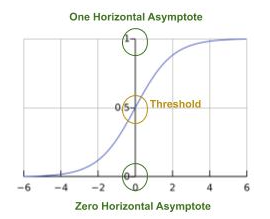
\includegraphics[width=2.8075in,height=2.2811in]{./media/Pictures/100002010000010E000000DBBE8AE7CA978D50DF.png}

\textbf{Feature Removal}

Data sources used in linear/logistic regressions typically are in the
form of structured data, also known as tabular, which originated from a
database. The dataset will consist of rows, each example, and columns,
where one column is the label and the remaining are the features.

It's not unusual when data comes from a database that it contains
columns which are not useful, or may even inhibit the training of the
model, and these types of columns need to be eliminated (removed) prior
to training. This is especially the case, if one used a SELECT * in an
SQL query, which would retrieve all columns.

Some typical examples of columns (features) we want to eliminate either
at the time the dataset is extracted from the database or after it's
extracted:

\begin{itemize}
\tightlist
\item
  It's common for each entry (row) in a database table to have a unique
  identifier, which may be a cardinal ordering like 1, 2, 3, etc., and
  typically is named something like ``Id''. This column is not otherwise
  part of the data and needs to be removed.\\
\item
  It's somewhat common for each entry to have a timestamp on when the
  entry was added to the database, and is typically named something like
  ``created'' or ``updated''. This column is not otherwise part of the
  data and needs to be removed.\\
\item
  Sometimes a database table has a text column for a note or other
  commentary, that is typically added by a person whom either created
  the data or entered it. While the column (field) potentially may have
  information relating to the data, for regression analysis one
  typically discards all textual data that is not categorical in nature.
\end{itemize}

\textbf{Feature Transformation}

\emph{Linear/logistic regression} analysis take datasets that consist of
numbers, specifically real numbers. Datasets therefore need to be
prepared prior to being used for training. This preparation maybe part
of a preprocessing phase, hand done, or automated in an extract
transform load (ETL) process.

In \emph{linear/logistic regressions}, the independent variables
(features) must be either continuous or discrete, which are also
referred to as numeric and categorical, respectively. In some cases, the
(representational) format of the independent variable is neither, and
must be transformed into either a continuous or discrete value.

Sometimes it may not be obvious when an independent variable is
continuous. Take the measurement of time, and assume it's format is
MM-DD-YY:hh:mm:ss. As is, we can't use it. If we convert the time into
an ordinal representation, such as the number of seconds since Jan 1,
1970, we then have a continuous value. This is an example of a
\emph{feature transformation}.

It's also common for independent variables that are meant to be a
discrete value to be in a format that is not a representation for a
discrete value, and will require a \emph{feature transformation}. In
most cases, discrete variables will fall into one of the following
types:

\begin{itemize}
\tightlist
\item
  Binary
\item
  Multi-Categorical
\item
  Bins
\end{itemize}

A binary value needs to be transformed into the value 0 and 1,
respectively. Thus, if the format of the value is textual such as True
and False, it will have to be transformed into it's discrete value
representation.

In the past, it was not uncommon for a categorical value which only had
two categories (i.e., distinct labels) to transform it into a binary
discrete representation (i.e., 0 or 1). For example, this was once a
common practice for gender, where male was transformed into 0 and female
into 1. I am sure you see the potential problem. What happens if in the
future the definition for the independent variable goes from two
categories to multiple categories. As in our example, it's now a common
practice to represent gender as a multiple categorical representation,
which we discussed next.

A multi-categorical, commonly shortened to categorical, value has two or
more categories. For example, a value which can be one of: blue, green
or brown (e.g., eye color) would be categorical, or a value which could
be one of the 50 USA states. Categorical values are transformed into
binary values, one per category. Using our example of eye color, one
would transform the single feature into three binary features:

eye\_color \{ blue, green, brown \} =\textgreater{} eye\_color\_blue \{
0, 1 \},\\
eye\_color\_green \{ 0, 1\},\\
eye\_color\_brown \{ 0, 1\}

The transformation of a categorical feature into a set of binary
features is also referred to as dummy variable conversion. The term
dummy is used to indicate that the transformed binary values are
replacements of the non-numeric values, representing the presence or
absence of the categorical value. Recall, that \emph{linear/logistic
regressions} take as input real numbers, so if we use categorical
features, we must transform them.

It is also a common practice that when transforming the categorical
values to a set of binary values, to drop one category to avoid
multicollinearity, which is where one feature perfectly predicts
another. This is also referred to as the dummy variable trap.

For example, if the categorical feature gender was the values male and
female, and we converted into binary features male and female, then the
value of either one will perfectly predict the value of the other. By
dropping one category from the transformation, one eliminates
multicollinearity, and the drop categorical value is implicitly
represented by all the remaining transformed binary features being
false. That is, if all the explicit binary features are false, then the
implicit binary feature is true.

Using the earlier example for eye color and dropping one category, such
as brown, we would have for a transformation:

eye\_color \{ blue, green, brown \} =\textgreater{} eye\_color\_blue \{
0, 1 \},\\
 eye\_color\_green \{ 0, 1\}

where eye\_color\_brown = (eye\_color\_blue == 0 and eye\_color\_green
== 0)

A bin, also referred to as a bucket, are ranges of real values, which
might appear initially continuous, but are actually discrete values
because their relevance is when they are grouped together, also referred
to as bucketization. That is, all the values within a bin (group) have
multicollinearity, in that they predict each other, and are replaced by
a single discrete value. For example, presume we are trying to find the
correlation between the independent variable a person's age and the
dependent variable what the person spent. One would break age into bins
for the following reason:

infant (\textasciitilde{}0 .. 2): they don't know meaning of money so
spending \textasciitilde{}0.\\
preschool (\textasciitilde{}3 .. 5): they spend the pocket change
parents give them.\\
elementary (6..11): they spend money earned from allowance and chores.\\
secondary(12..17): they spend money earned from chores and odd jobs.\\

\textbf{Feature Normalization}

The process of \emph{feature normalization} occurs once all
\emph{feature transformations}, and \emph{feature engineering} (not
discussed in primer) are completed. \emph{Feature normalization} is
performed on the features that are continuous, also referred to as
numeric. The purpose of normalization is to prevent the numeric range
and distribution of one feature to overly dominate other features with
smaller ranges and narrower distributions. Without normalizations,
training may take longer and may not converge
(\href{https://github.com/GoogleCloudPlatform/keras-idiomatic-programmer/blob/master/handbooks/The\%20Idiomatic\%20Programmer\%20-\%20Learning\%20Keras\%20-\%20Handbook\%202\%20-\%20Computer\%20Vision\%20Data\%20Engineering.pdf}{not
discussed in primer}).

Let's start with an example. Let's assume we are doing a \emph{multiple
linear regression }where one will predict spending (dependent variable),
and the independent variables are years of education, and employment
income (not investment). From exploring the data prior to performing the
analysis (training), we find the following range, the minimum and
maximum values, of the two independent variables:

years\_of\_education : 8 ... 27\\
income : 12,000 .. 1,500,000

If your wondering why we chose 27 for the maximum value of years of
education, we choose it due to doctors in the USA typically do 4 years
undergraduate, 4 years in medical school and 3 to 7 years residency.\\
~\\
Here's the problem, the range for income way over dominates that of
years of education. We have 1500 and 55K times greater than on the
minimum and maximum, respectively. During training, one will want to
gradually learn the best fitted weights for w\textsubscript{1} (years of
education) and w\textsubscript{2} (income). When training starts, we
don't know what the final value of the weights will be, so they are
initialized by some algorithm to typically a very small value. After
feeding a batch of examples (not discussed in primer), the loss is
calculated and the weights are updated to reduce the loss on the next
batch, also referred to as minimizing.

In our example, as is, the contribution to the loss function from the
feature income will dominate that of the years of education,
disportionality influencing the updating (learning) of the weights. The
\emph{multiple linear regression} will spend a considering amount of
time learning the correct correlation between years of education and
income before being able to learn the correct weights (contribution). If
it does not learn the former, the training will never converge -\/-i.e.,
won't be able to fit a correlation between the independent variables and
dependent variables.

We approach this problem using \emph{feature normalization} (also
referred to as feature scaling), where we squash the range of each
continuous (numeric) feature into the same range, typically between 0
and 1. The equation below performs a scaling between 0 and 1:

\begin{quote}
\end{quote}

\begin{quote}
x\textsubscript{i}' = {}
\end{quote}

\begin{quote}
\emph{x}\textsubscript{\emph{i}}\emph{ } : the unscaled value of an
instance (example) in feature set \emph{x}.\\
\emph{x}\textsubscript{\emph{i}}\emph{'} : the scaled value of an
instance in feature set \emph{x}.\\
\emph{min(x) }: the minimum value of all instances in feature set
\emph{x}.\\
\emph{max(x)}: the maximum value of all instances in feature set
\emph{x}.
\end{quote}

Once the continuous features have been normalized, we do not need to
first learn the correlation between the features, and simply now just
learn how the features correlate to the dependent variable. The training
will more likely converge and in shorter amount of time.

Beyond the method described above, there are other methods for
\emph{feature normalization}. Another method, which is the common
practice is \emph{feature standardization}. In \emph{feature
standardization}, we first scale the values within a range (like -1 and
1), and then from within the range we use the distribution of the values
to redistribute the values centered on a mean of zero and standard
deviation of one.

The objective here is to improve convergence and further lessen the time
to train a linear/logistic regression (and other types of models) by
making all the independent features share a similar distribution in
values. We accomplish this using a principle from the central limit
theorem, that regardless of the population distribution, if we plotted
the mean of random samples, the means would form a normal distribution.

The method of \emph{feature standardization} remaps the scaled values
into a normalized distribution, for each independent continuous feature.
The equation below performs a standardization:\\

\begin{quote}
x\textsubscript{i}' ={}
\end{quote}

\begin{quote}
\emph{x}\textsubscript{\emph{i}}\emph{ }: the unstandardized value of an
instance (example) in feature set \emph{x}.\\
\emph{x}\textsubscript{\emph{i}}\emph{'} : the standardized value of an
instance in feature set \emph{x}.\\
{}\emph{ }: the mean of all instances in feature set \emph{x}.\\
{}: the standard deviation of all instances in feature set \emph{x}.
\end{quote}

\protect\hypertarget{anchor-20}{}{}

\protect\hypertarget{anchor-21}{}{}\textbf{Part C - CART Analysis}

CART is an acronym for \emph{Classification and Regression Trees}. The
term is attributed to a publication of the book by Brieman, et. al, in
1984 titled Classification and Regression Trees. The objective of CART
is to find methods to model non-linearity of features that contribute to
the predicted outcome. As we discussed earlier, the \emph{linear
regression} and \emph{logistic regression} models predict well when the
independent variables are correlated to the predicted value (real value
or classification), and the independent variables have a linear or
logistic relationship to the dependent variable.

CART analysis introduced a methodology to predictive modeling to address
independent features which contributed significantly to the prediction
(outcome) but did not correlate to the dependent variable in a linear or
logistic relationship. What CART addressed is the assumption that in
these cases, the independent variables did exhibit linear or logistic
relationships but in segments over their discrete or continuous value
ranges vs. across the entire range.

CART addresses this type of relationship between the independent
variable(s) and the dependent variable through decision trees. Unlike
a\emph{ linear/logistic regression} which learns weights for how an
independent variable is correlated to the dependent variable in a linear
or logistic manner, it learns thresholds to segment the correlations
into subsets of linear or logistic correlations.

Let's take the example of age and spending. As discussed previously, we
can segment age into ranges that do not have a linear/logistic
relationship across the segments, but do have such a relationship within
the segmented age range. The premise behind CART is to learn these
``decision boundaries'' to segment the independent variables, such that
within the segment the relationship to the dependent variable continues
to be linear or logistic.

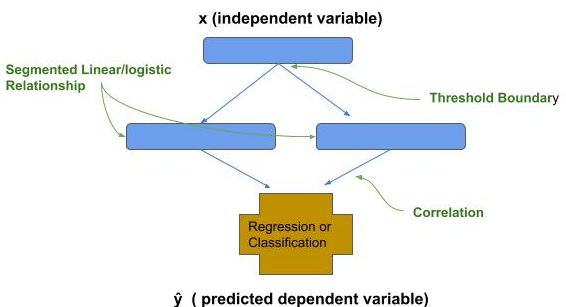
\includegraphics[width=5.3598in,height=2.9055in]{./media/Pictures/100002010000023600000133934F4973A049ED43.png}

The above depiction illustrates an example where the range of values for
the independent variable \emph{x} does not have a linear/logistic
relationship to the dependent variable \emph{y}. In the example, a
threshold is learned that splits the range of values, referred to as a
decision split, into two groups; whereby within each group the values of
the independent variable does have a linear or logistic relationship to
the dependent variable.

Since CART analysis does not assume a linear/logistic relationship, it
is a useful technique when the relationship between the independent
variables and dependent variable is not linear/logistic.

\textbf{Decision Trees}

CART analysis is based on building decision trees. Decision trees
consist of nodes, threshold, branches and leaves. Each node is
associated with a single independent variable. The threshold is a value
within the range of the independent variable (or function applied to
independent variable) that separates the data into two independent
groups; whereby each of the two groups has higher homogeneity
individually than combined. Higher homogeneity means that the values
have higher correlation to the dependent variable. The branches direct
the splitting to the next node in the decision tree. A leaf is a node
that has no further split. The leaf is either a final predictor or part
of a set of predictors, such as in an ensemble method (to be discussed
subsequently).

Decision trees are assembled as either \emph{regression trees }or
\emph{classification trees}, where a \emph{regression tree }predicts a
continuous value (i.e., regressor) and a \emph{classification tree
}predicts a discrete (categorical) value (i.e., classifier).

The basic method for making a decision tree nobody does anymore, so we
will cover it very briefly. One takes the set of independent variables
(features) and ranks order them according to how well the independent
variable is correlated to the dependent variable. Then you make a tree
where the root is the highest correlating feature. At the next level
down (level 2), you add a decision node on both branches which is the
next highest correlating feature, at the next level all the decision
nodes use the next highest correlating feature of the remaining
features, and so forth. For example, if there were 10 features, the
highest correlating feature would appear as a single node at the root
and the lowest correlating feature would have 4096 decision nodes at the
leaves of the tree, where the number of nodes is 2\textsuperscript{n-1},
where n is the number of features, such as depicted below:

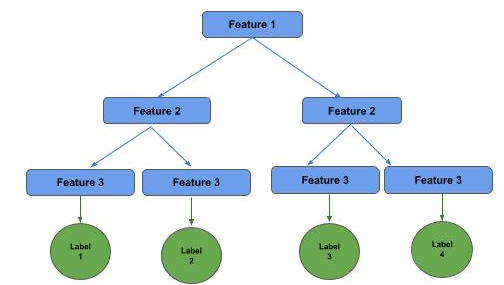
\includegraphics[width=5.25in,height=2.9689in]{./media/Pictures/10000000000001F80000011D64B897CC6C5A4AB3.png}

Popular methods of the time for ranking ordering the features were using
information gain (not discussed in this primer) for features that are
categorical and gini index (not discussed in this primer) for features
that are continuous.

Due to the enormous amount of training required and exposure to
overfitting, decision trees fell out of favor for a period of time. In
the last ten years, several new techniques have been developed that
substantially reduce tree size, reduce training and increase accuracy,
including ensemble, bagging and boosting. As a result, CART analysis
re-emerged as part of modern machine learning.

\textbf{Ensemble (Weak Learners)}

Decision trees became popular again when the ensemble method was applied
to constructing decision trees. An ensemble is not a single model (e.g.,
decision tree), but a collection of computationally smaller models;
whereby, each model is assumed to be 50\% or better in accuracy. These
smaller models are also referred to as weak learners. The assumption is
that as we combine more weak learners, then the combined decision (e.g.,
majority voting in logistic classification), the more accurate the
prediction will be. This concept is based on the seminole work in 1785
on jury systems by French mathematician Marquis de Condorcet, titled
\emph{Essay on the Application of Analysis to the Probability of
Majority Decisions. }In his essay, Condorcet proposed a mathematical
proof that if each person in a jury is 50\% or better at the correct
decision, then the more people added to the jury, the probability of the
correct decision increases. Likewise, his mathematical proof also
demonstrated that if each person in a jury is less than 50\% at getting
the correct decision, then the more people added to the jury, the
probability of the correct decision decreases.

For example, if the ensemble is for a logistic classifier, then the
method for a combined decision maybe a majority vote. If the ensemble is
for a linear regressor, then the method maybe the mean.

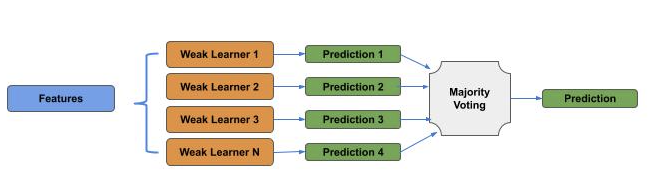
\includegraphics[width=6.5in,height=1.7917in]{./media/Pictures/100002010000028F000000B45484410EACF1F151.png}

\textbf{Bootstrapping}

Bootstrapping is a method for improving the estimate of the mean of a
population distribution from a single sampling. For example, let's
assume our population are shoe sizes of men in North America, and we
have a single sample of 10,000 random instances (examples). We can
calculate the mean of the single sample, but since it was a single
sample, we cannot create a sampling distribution and use the central
limit theorem to approximate the actual mean and standard deviation.

To better improve our approximation from a single sample, we randomly
resample from our sample to create new samples. That is, if our sample
size was N, we make new samples of size N, but randomly draw instances
(examples) from the original sample. Since the draws are random, we are
likely to have some duplicated instances in the resampled sets, but with
sufficient size N, each resampled set is likely to be unique. Below is
an example:

Sample = {[}1, 2, 3, 4, 5{]}\\
Resample 1 = {[}2, 4, 2, 5, 1{]}\\
Resample 2 = {[}5, 5, 1, 4, 3{]}

The principle here is that each resample has a 50\% or better chance of
being an actual sample in the population, and as such, using ensemble,
the more samples we generate through resampling, the more accurate our
calculation of the mean and standard deviation of the population will
be.

\textbf{Bagging}

Bagging (short for Bootstrap Aggregation) is an ensemble method, which
uses an ensemble of models, trained on smaller resampled training data,
where the resampling is based on bootstrapping, and the aggregation
refers to the combined decision method, e.g., majority voting if
logistic classifier.

For example, assume a training dataset has 10,000 instances, where we
refer to the size of the training data as \emph{n}. We first choose a
resampling size \emph{n' }(n prime), which is smaller than \emph{n},
such as 60\% in size. We then select the number of resampled training
sets as \emph{m}, where each resampled training set is referred to as a
bag. We then train \emph{m} models, one per resampled training set, and
then combine the prediction of each model in an ensemble method, where
the assumption is each model trained on the smaller resampled dataset is
a weak learner (i.e., 50\% or better accuracy).

For example, in a categorical classifier, one would combine (additive)
the probability distribution of the predicted classes (labels) prior to
passing through a softmax activation function for an aggregated
probability distribution.

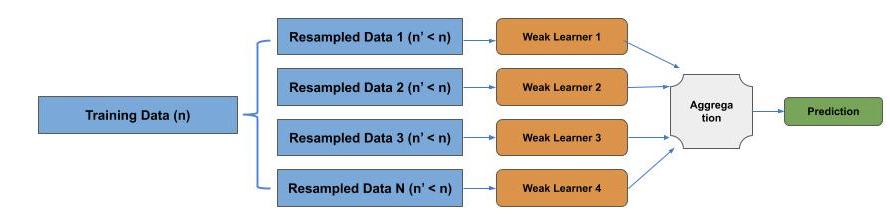
\includegraphics[width=6.5in,height=1.5693in]{./media/Pictures/100002010000037A000000D627941350EE03BCFA.png}

\textbf{Random Forest}

A state-of-the-art application of the bagging method to decision trees
is the Random Forests (trademarked) method. In Random Forests, instead
of resampling the training data, the features (independent variables)
are resampled, which is also referred to as feature bagging. Assuming we
have \emph{p} features, then each resampled feature set is of size
\emph{p'}, where \emph{p'} is smaller than \emph{p}.

For example, assume our training set has 16 features, which we refer to
as \emph{p}. We then choose a feature resampling size, such as 4, which
we refer to as \emph{p'}, where \emph{p'} {} {} is the general practice.
Next, we select the number of models as \emph{k}.

For each model (decision tree), we randomly select the \emph{p'}
features from the set of \emph{p} features. Each model has a random
distribution of features, but are likely to have overlap of some
features with one or more models.

The random selection of features is used to prevent the models from
being highly correlated. That is, the more similar the models are, then
any model becomes a predictor of the other models. Instead, we want each
model to be an independent predictor (uncorrelated).

Finally, for each model (decision tree), we generate a resampled dataset
from the training set using bootstrapping. That is, the size of the
resampled datasets are the same size as the training set, but each
decision tree is trained on a randomly chosen resampling. Each model is
a decision tree, and the ensemble of decision trees is a forest.

Finally, we combine the prediction of each model in an ensemble method,
where the assumption is each feature bagged model trained on a resampled
dataset is a weak learner (i.e., 50\% or better accuracy).

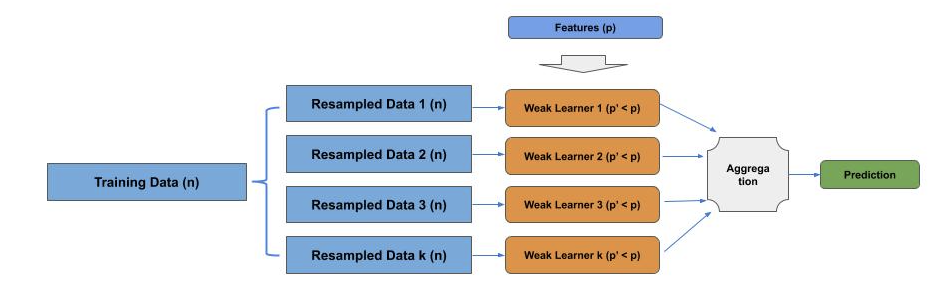
\includegraphics[width=6.5in,height=1.9445in]{./media/Pictures/10000201000003AC0000011A431350B1B448308E.png}

\textbf{Boosting}

Boosting is a method for turning weak learners into stronger learners
(i.e., boosting a weak learner into a stronger learner). In this method,
one takes an ensemble of weak learners, whose prediction accuracy is
otherwise only slightly better than random guess, and then boost each
weak learner to be more correlated with the correct predictions.

Boosting algorithms use some form of re-weighting of the models and/or
training data. In earlier non-adaptive versions of boosting, the general
practice was to weight the contribution to the final prediction by its
accuracy on the test data. For example, if one had models A, B and C
with corresponding accuracies on the test data of 51\%, 54\% and 57\%,
then the prediction of model A would contribute 51\% to the final
prediction, model B would contribute 54\% and finally model C would
contribute 57\%.

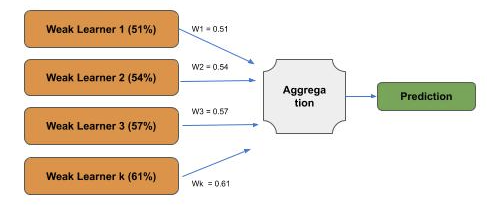
\includegraphics[width=5.0728in,height=2.1874in]{./media/Pictures/10000201000001E7000000D27AC3951B4C17C2E0.png}

Conventional boosting methods use some form of adaptive boosting. The
principle is that each new weak learner focuses on improving on training
data that was misclassified by the previous weak learner; which is
typically referred to as reweighting the training data.

For example, after training a first weak learner, we would identify the
training data examples which were misclassified. In the next weak
learner, the misclassified examples in the (resampled) training data are
given a higher weight, such that they have a higher loss (i.e., greater
penalty) then the previous correctly classified training examples. This
causes the adjustments to the new weak learner to focus (be biased
towards) the previous misclassified training examples. The process is
then repeated for the next weak learner.

There are a variety of methods to re-weighting the training data. In one
method, we bias the resampling to cause an increase in the number of
occurrences of the misclassified training examples from the training
dataset.

\textbf{AdaBoost}

In a second example, referred to as AdaBoost,we add a weight (i.e.,
greater than one) to the misclassified examples which is applied to the
cost calculation when the predicted value does not equal the actual
value. For example, if the weight is 1.2, then the cost calculation on
misclassification is multiplied by a factor of 1.2.

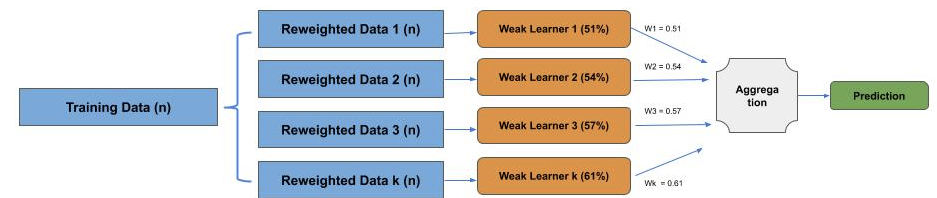
\includegraphics[width=6.5in,height=1.3752in]{./media/Pictures/10000201000003A9000000C618E7F15452ED9990.png}

\protect\hypertarget{anchor-22}{}{}\textbf{Part D - Probabilities}

In this part, we cover the fundamentals of independent and conditional
probabilities.

\textbf{Independent Probabilities\\
~\\
}An independent probability is when the probability of any instance of
an event has no dependence on a prior event. A common example of an
independent probability is a coin toss for heads vs. tails. We know that
on any given coin toss, the probability of heads (A) is 50\%, and
conversely the probability of tails (B) is 50\%. We can represent this
with the following formulazitation:

\begin{quote}
\emph{P(A) = 0.5\\
P(B) = 1 - p(A)}
\end{quote}

In the above \emph{P() }represents a probability of an event specified
by the parameter. Thus, \emph{P(A) }reads as the probability of event A
(e.g., coin toss is heads) being true. In an independent probability,
the inverse of the event is directly correlated to the event. So in the
case of a coin toss which has just two outcomes (heads or tails). The
probability of the inverse of the event, where \emph{P(B) }is the
probability of event B being true (e.g., tails), is 1 - the probability
of the event.

In an alternate notation, P() is denoted as \emph{P{[}{]}}, where the
above would be represented as:

\emph{P{[}A{]} }= 0.5\\
P{[}B{]} = 1 - \emph{P{[}A{]}}

In an independent probability, if we keep repeating the event, the
aggregation of the events will eventually equal that of a single
instance of an event. For example, if we toss the coin ten times, the
average of the results maybe 60\% heads, 40\% tails (i.e., 60/40). But
as we continue to toss the coins, we increase the likelihood that the
aggregation will approach and equal that of a single event.

In other words, each instance of the event is uncorrelated from every
other instance. Thus, each individual instance of the event (coin toss)
will be an independent probability, but the aggregation of increasing
events will approach or equal the probability of a single event.

\textbf{Random Walk}

A random walk is a probability method based on independent
probabilities. A random walk is a random process of equal length steps,
which is typically represented by integers. The sequence starts at an
origin labeled 0, followed by a sequence of steps. At each step, there
is a set of equal length actions that can be selected from. For example,
if the random walk is along a line, at each step one can go either
negative distance (left) or positive (right). On a 2D space, one might
define the steps as the Manhattan distance (up, down, left, right). At
each step, a random choice is made from the set of actions.

\emph{\textbf{Line}}

Let's look at an example when the random walk is along a line. Assume we
have a random number generator which produces a uniform random
distribution of choices of -1 and 1, and produced the following ten step
distribution:

{[}1, -1, -1, 1, -1, 1, -1, -1, -1, 1{]}

If we plot this as steps, we have the following location on the line at
each step:

Step 1: 1\\
Step 2: 0\\
Step 3: -1\\
Step 4: 0\\
Step 5: -1,\\
Step 6: 0,\\
Step 7: -1,\\
Step 8: -2,\\
Step 9: -3\\
Step 10: -2

We repeat several times using the same uniform random number generator
for 1000 steps, and have the following position at the last step, and
the greatest distance at any step:

Last Position Absolute Greatest Distance

-12, 39\\
28, 51\\
4, 9\\

As you can see, given a uniform random distribution, we never venture
that far from the origin.

\emph{\textbf{Manhattan Distance}}

Let's assume a 2D grid and at each step we can move up, down (vertical)
or left, right (horizontal). We will represent the horizontal and
vertical movements as x and y, respectively. At each step, we can
randomly choose to take one step from the four choices -\/- this is
sometimes known as the ``drunken man walk in city streets''.

\begin{quote}
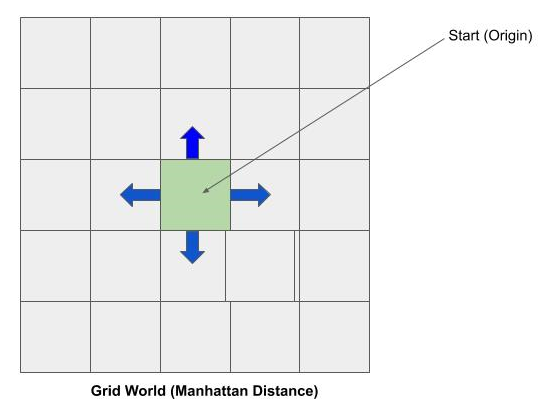
\includegraphics[width=4.1047in,height=3.1339in]{./media/Pictures/100002010000021D0000019D8B2B9690F1068763.png}
\end{quote}

We repeat this three times using a uniform random number generator for
1000 steps, and have the following x, y position at the last step:

(-6, -42)\\
(16, 6)\\
(-30, -28)

Again, notice that after a 1000 steps, we have not moved far from the
origin. Random walks are used for modeling stochastic movements using a
random distribution, such as modeling a molecule moving through a liquid
or gas, fluctuations in a stock price, etc.\\
~\\
\emph{\textbf{Gaming}}

Random walks are also used in gaming. For example, let's design a game
that consists of a box of four walls, and within the four walls is a
grid. You start at some origin zero, and at each step you must make a
choice to move up, down, left or right. If you don't move you are
incinerated by an alien ray gun. At the same time, a lion is randomly
moving through the grid. If you move into a block where the lion is, you
are eaten. Using the random walk principle, it's likely at any move you
won't stray too far from the origin or otherwise return to the origin.
If I program the lion to do a grid walk in a smaller grid area around
the origin, chances are it won't be long before you're eaten -\/-game
over.

When I was in grad school, I wrote a computer game for HP scientific
calculator called Gunboat Diplomacy. The overall rules were simple.
There were six sets of islands, the first and last set had one island
and the sets between had three islands. You started at the first island
and the goal was to make it to the last island. You started with and
could carry a maximum of three ammo packs. On each turn, you had a
reconnaissance where you could choose to see the number of enemies on
one island only, either forward, backward or laterally. It took one ammo
pack to kill an enemy and an island never had more than two enemies. You
could move backwards to refresh your ammo packs. Seems simple, easy to
beat. My grad friends played the game for days, weeks and months and
never won. I could play the game and show you can win. My super-brainy
friends could not figure out why -\/-I never told them it was based on
random walks. You figure the rest out.

\textbf{Part D - Conditional Probabilities}

A conditional probability is where the probability of an event is
dependent on a past event, or existence of another event. This form of a
probability is denoted as:

\emph{P(A\textbar{}B)}\\

In the above, the event A is the event we are determining a probability
for being true, and B is the existence of an event B. This can be read
as: what is the probability of A being true, when B is true. The above
is sometimes denoted as:

\emph{P{[}A\textbar{}B{]}\\
}

For example, one might predict the probability of missing the bus when
the alarm clock does not go off. In this example, the event A (what we
are predicting) would be ``missing the bus'', and event B (what is true)
would be ``alarm clock does not go off''. We could write this as:

\begin{quote}
\emph{P(miss the bus \textbar{} alarm clock does not go off)\\
}
\end{quote}

For another example, let's look at predicting if someone has cancer.
First, we could look at it as an independent probability -\/-i.e.., not
dependent on any other event or information. We could represent this as:

\begin{quote}
\emph{P(has cancer)}
\end{quote}

\begin{quote}
\end{quote}

Now let's change this and add that you took a cancer test. The test is
not perfect. For some people it will predict you have cancer when you
don't (false positive) and at other times it will predict you don't have
cancer when you do (false negative), and there is a known probability
distribution for the false positive and false negative. In this case, we
now have a conditional probability where we predict if you have cancer
when your cancer test is positive, which can be denoted as:

\begin{quote}
\emph{P(has cancer \textbar{} test is positive)\\
}
\end{quote}

\textbf{Monty Hall Game Show Paradox}

The Monty Hall Game Show Paradox is one of my favorite ways to
demonstrate the difference between an independent and conditional
probability. I like it, in that to the general public, inclusive of
PhDs, they assume it's an independent probability and get the wrong
answer. It is a conditional probability.

The problem (or puzzle) is based on the game show Let's Make a Deal,
originally hosted by Monty Hall. The problem was first posed and solved
by the statistician
\href{https://en.wikipedia.org/wiki/Steve_Selvin}{Steve Selvin} in a
letter to the
\href{https://en.wikipedia.org/wiki/The_American_Statistician}{American
Statistician} in 1975. It became famous in a readers letter to
\href{https://en.wikipedia.org/wiki/Marilyn_vos_Savant}{Marilyn vos
Savant}'s "Ask Marilyn" column in
\href{https://en.wikipedia.org/wiki/Parade_(magazine)}{\emph{Parade}}
magazine in 1990:

Suppose you're on a game show, and you're given the choice of three
doors: Behind one door is a car; behind the others, goats. You pick a
door, say No. 1, and the host, who knows what's behind the doors, opens
another door, say No. 3, which has a goat. He then says to you, "Do you
want to pick door No. 2?" Is it to your advantage to switch your choice?

Marilyn vos Savant's answer was that it was better to pick another door,
in that you'd have a ⅔ chance of winning the car, and only ⅓ chance if
you stuck with the same door. After Marilyn vos Savant's response was
published in Parade magazine, the magazine received 10,000 responses
that she was wrong, with nearly 1000 with PhDs, where the responders
argued that the probability did not change -\/-that is, in both cases
the probability of winning the car was ⅓.

Vos Savant was correct, because the problem (puzzle) is a conditional
probability, while the respondents presumed it was an independent
probability. The respondents viewed the problem that each door had a ⅓
chance of having the car, and that there was no dependency between the
doors; therefore, changing to the other remaining door should have the
same ⅓ chance.

The respondents looked a dependency, which was not missed by vos Savant.
She correctly say that by the host (i.e., Monty Hall) eliminating a door
which he knew did not have the winning car, created a conditional
dependency. Had the problem been stated that the host opened one of the
two remaining doors without knowing if they had the winning car, and
thus could end up opening a door with the winning car, it would've then
been an independent probability, as the respondents argued.

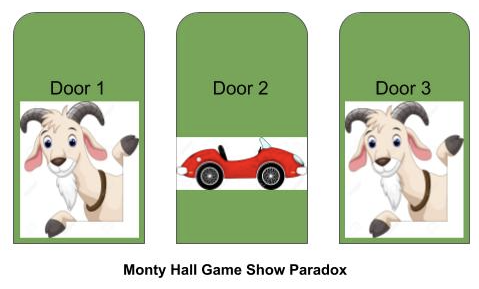
\includegraphics[width=3.911in,height=2.3598in]{./media/Pictures/10000201000001DF00000121D02265BF9DB69DF9.png}

\begin{quote}
\href{https://www.123rf.com/photo_34715770_stock-vector-cute-goat-cartoon.html}{\emph{Goat
License}} -
\href{https://www.123rf.com/photo_20679360_funny-red-convertible-car-cartoon-isolated-on-white-background.html}{\emph{Car
License}}
\end{quote}

,

Let's look a little closer now at the problem. At the start, the
contestant does not know which door has the car; so irregardless of the
door they first selected, it has a ⅓ chance of being the car -\/-hence
without any other event, this is an independent probability. While the
contestant's door has ⅓ chance of the car, the remaining two doors
combined have the remaining ⅔ chance.

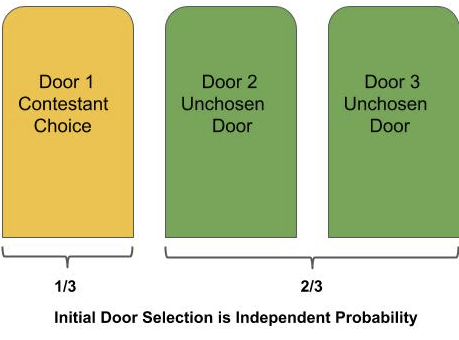
\includegraphics[width=3.4016in,height=2.5201in]{./media/Pictures/10000201000001CB00000154FF490A1CB5D13E50.png}

Now, while the contestant doesn't know what's behind each door, the host
(Monty Hall) does know. Regardless of whether the contestant first
chance is the winning choice, at least one of the remaining two doors is
a non-winning door. That is, if the first choice is the winning door,
both the remaining doors are non-winning doors, and if the first choice
is not the winning door, then one of the remaining doors is the winning
door and the other is a non-winning door.

Since the host has the knowledge, and will open only one of the
remaining doors that is a non-winning door, the selection is
conditionally dependent on the host's knowledge. Thus, the probability
of the two remaining doors combined, a non-winning door which has been
opened and the other unopened door is still a ⅔ chance of winning. But
since a non-winning door of the two remaining doors were opened, the ⅔
chance of winning is transferred to the other unopened door.

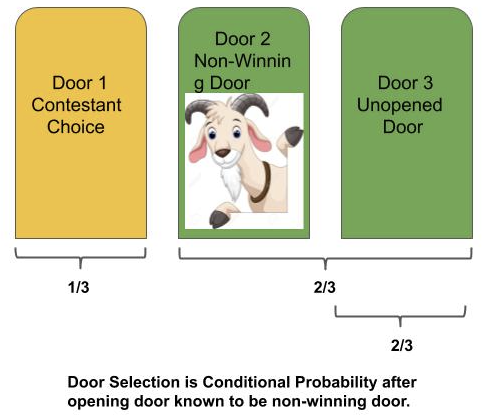
\includegraphics[width=3.3902in,height=2.9173in]{./media/Pictures/10000201000001E4000001A25B6BAFAA1E0C65A4.png}\\

If your still skeptic, then you can prove it empirical. Use a
spreadsheet. You will have nine rows, three for each door, one for the
for the door being the winner, and the other two rows for each of the
other two doors being the winner. Add one column for sticking with the
door, and one column for choosing the remaining unopened door. Calculate
the probability for each cell. Then aggregate the probability for
sticking with the initial selection, which will be ⅓, and aggregate the
probability for switching choice to the unopened door, which will be ⅔.
I will leave it up to you to build the spreadsheet and prove to yourself
empirically if you're still skeptical.

\textbf{\\
Bayes Theorem}

Bayes theorem is the defacto standard for conditional probabilities. In
the base form, the theorem is represented as:

\emph{P(A\textbar{}B) = }{}

The above can be expressed as follows, if we know the independent
probabilities of the events A and B being independently true,\emph{
P(A)} and \emph{P(B)}, then we can determine the conditional probability
of A being true when B is true -\/- \emph{P(A\textbar{}B)}, if we know
the inverse conditional probability of B being true when A is true -\/-
\emph{P(B\textbar{}A)}.

In the above P(A) and P(B) are referred to as the prior (i.e., your
prior knowledge). Let's demonstrate with an example. Assume we want to
determine the probability of an email being spam (A) given the presence
of some specific text sequence (B), which we represent as:

\emph{P(A\textbar{}B) = P(spam\textbar{}specific text sequence)}

Let's say we have the prior knowledge of knowing the percentage of
emails that are spam, independent of the contents of the email. We will
call that the \emph{P(A),} which in our example we denote as
\emph{P(spam) }and say that it is 1 in 100 emails, or 0.01. Let's say
that we know the probability that the specific text sequence occurs in
an email, We will call that\emph{ P(B)}, which in our example we denote
as \emph{P(specific text sequence)} and say that it is 1 in 1000 emails
or 0.001:

\emph{P(A) = P(spam) = 0.01``\\
P(B) = P(specific text sequence) = 0.001}

Now let's say we know the probability of an email that is spam contains
the specific text sequence. We will call that P(B\textbar{}A), which in
our example we denote as P(specific text sequence\textbar{}spam) and say
that it is 1 in 50 spam emails, or 0.02.

P(B\textbar{}A) = P(specific text sequence\textbar{}spam) = 0.02

Let's now calculate the probability that an email is spam given the
presence of the specific text sequence. Putting it altogether, we have:

{}= 0.20

That's Bayes, we hope you enjoyed our statistics primer, and look
further into our AI Primer and NLP Primer.
